\documentclass[a4paper,12 pt,twoside]{report}
\usepackage{fullpage}

\usepackage{mystyle}


\begin{document}

\begin{titlepage}

  % AUTH Logo
  \begin{minipage}{0.3\textwidth}
    \begin{flushleft}
      
\includegraphics[scale=0.25]{./images/title/authLogoTr.jpg}
    \end{flushleft}
  \end{minipage}
  \begin{minipage}{0.9\textwidth}
    \begin{flushleft}
      \large Αριστοτέλειο Πανεπιστήμιο Θεσσαλονίκης \\
      Πολυτεχνική Σχολή \\
      Τμήμα Ηλεκτρολόγων Μηχανικών $\&$ \\ Μηχανικών Υπολογιστών\\

      \normalsize{Τομέας Ηλεκτρονικής και Υπολογιστών} \\[5cm]
    \end{flushleft}
  \end{minipage} \\[1.7cm]




  \begin{center}
    \Large Διπλωματική Εργασία \\[0.8cm]

    \rule{450pt}{4pt} \\[0.4cm]
    {\fontsize{20.26pt}{1em}\selectfont Έρευνα ταξινομητών DNN για αναγνώριση αντικειμένων και βελτιστοποίηση για το ενσωματωμένο σύστημα Jetson-TK1}

    \rule{350pt}{4pt} \\[4cm]

    % Writer
    \begin{minipage}{0.4\textwidth}
      \begin{flushleft} \large
        \emph{Εκπόνηση:} \\
        Παναγιώτου Κωνσταντίνος \\
        ΑΕΜ: 7316
      \end{flushleft}
    \end{minipage}
    % Supervisors
    \begin{minipage}{0.4\textwidth}
      \begin{flushright} \large
        \emph{Επίβλεψη:} \\
        Αν. Καθ. Πέτρου Λουκάς\\
        Υπ. Δρ. Μουσουλιώτης Παναγιώτης \\
        %Δρ. Τσαρδούλιας Εμμανουήλ
      \end{flushright}
    \end{minipage}
    \\[1cm]
    \vfill

    % Title
    \large Θεσσαλονίκη, Σεπτέμβριος 2016

  \end{center}
\end{titlepage}


\newevenside

\pagenumbering{roman}
\thispagestyle{empty}
\mbox{}
\begin{flushright}

{\fontfamily{lmr}\selectfont
  \vspace{6cm}

  %\epigraphsize{\small\itshape}

  %\epigraph{And so it goes...}{--- \textup{Kurt Vonnegut}, Slaughterhouse Five}

  \it{
    The robots are going to help us find our crystal...
  }
}
\end{flushright}

\newevenside
\section*{Ευχαριστίες}
\phantomsection
\addcontentsline{toc}{section}{Ευχαριστίες}


Θα ήθελα να ευχαριστήσω θερμά τον καθηγητή κ. Λουκά Πέτρου
για την εμπιστοσύνη που μου έδειξε και την στήριξή του καθ᾽ όλη τη
διάρκεια της συνεργασίας μας, τόσο στην εκπόνηση την διπλωματικής
μου εργασίας, όσο και ως μέλος της ομάδας ρομποτικής P.A.N.D.O.R.A. του
τμήματος Ηλεκτρολόγων Μηχανικών και Μηχανικών Υπολογιστών
του Αριστοτελείου Πανεπιστημίου Θεσσαλονίκης.

Θα ήθελα επίσης να απευθύνω τις ευχαριστίες μου στον μεταδιδακτορικό
ερευνητή του τμήματος και φίλο Δρ. Εμμανουήλ Τσαρδούλια, καθώς και στον επιβλέποντα
και φίλο Υπ. Δρ. Παναγιώτη Μουσουλιώτη για την βοήθεια, τις συμβουλές και
την υποστήριξή τους· έμαθα πολλά από εσάς.

Το μεγαλύτερο ευχαριστώ το οφείλω στους γονείς μου Λάζαρο και Βασιλική καθώς
και στην αδελφή μου Έλενα για την στήριξη, τις θυσίες και την αγάπη τους όλα αυτά
τα χρόνια, δίνοντας μου κουράγιο να προχωρώ και να υπερπηδώ κάθε εμπόδιο
για να φτάσω στον στόχο μου.

Ένα εγκάρσιο ευχαριστώ αξίζει η φίλη και συνεργάτης Σοφία Ρέππου,
για την κατανόηση, την συμπαράσταση και την βοήθειά της τα τελευταία
χρόνια.

Τέλος, ευγνωμονώ συγγενείς, φίλους και γνωστούς για την όποια
συνεισφορά τους τόσο στην προσωπική όσο και την επαγγελματική μου πορεία
και τις όμορφες στιγμές και εποχές που μαζί περάσαμε.

\newevenside

\begin{center}
  \centering

  \vspace{0.5cm}
  \centering
  \textbf{\Large{Περίληψη}}
  \phantomsection
  \addcontentsline{toc}{section}{Περίληψη}

  \vspace{1cm}

\end{center}

  Η Μηχανική Μάθηση αποτελεί έναν από τους σημαντικότερους τομείς των τελευταίων
  ετών εξαιτίας της ανάπτυξης των Νευρωνικών Δικτύων.
  Εμπνευσμένα από τον τρόπο που λειτουργεί ο Εγκέφαλος και το Κεντρικό Νευρικό Σύστημα (ΚΝΣ)
  του ανθρώπου, αυτά τα υπολογιστικά μοντέλα ξεπερνούν προηγούμενες μορφές Τεχνητής Νοημοσύνης
  σε διαδικασίες μηχανικής μάθησης.
  Τα Νευρωνικά Δίκτυα Συνέλιξης (CNN) αποτελούν μία από τις πιο ενδιαφέρουσες μορφές αρχιτεκτονικής
  Νευρωνικών Δικτύων τα οποία χρησιμοποιούνται για την επίλυση προβλημάτων αναγνώρισης προτύπων
  στην Μηχανική Όραση (CV). Τα CNNs ανήκουν στην κατηγορία των αλγορίθμων εκμάθησης αναπαραστάσεων που
  σημαίνει ότι δεν απαιτείται η εξαγωγή χειρόγραφων (από τον άνθρωπο) χαρακτηριστικών για την αναγνώριση των
  προτύπων, ενισχύοντας έτσι τις μηχανές με την ικανότητα να εξάγουν μόνες τους
  τα κατάλληλα χαρακτηριστικά από μια δοσμένη εκ των προτέρων σειρά από δεδομένα.

  Τα ενσωματωμένα συστήματα έχουν περιορισμένη υπολογιστική ικανότητα σε σύγκριση με τα desktop και server συστήματα.
  Ωστόσο είναι σχεδιασμένα για εφαρμογές με χαμηλή ενεργειακή απαίτηση όπως
  είναι για παράδειγμα οι ρομποτικές εφαρμογές. Τα ρομπότ χρειάζεται να είναι εφοδιασμένα με την κατάλληλη 
  επεξεργαστική ισχύ που να τους επιτρέπει να πραγματοποιήσουν
  βασικές ενέργειες όπως είναι η πλοήγηση στο χώρο,
  η χαρτογράφηση και η αναγνώριση αντικειμένων χωρίς παράλληλα να καταναλώνουν
  τόση ενέργεια που να εξαντλεί το σύστημα.

  Η παρούσα Διπλωματική Εργασία εστιάζει στην υλοποίηση Νευρωνικών Δικτύων Συνέλιξης για την επίλυση θεμάτων αναγνώρισης
  αντικειμένων και εντοπισμού αντικειμένων στο ενσωματωμένο σύστημα Jetson TK1.
  Ερευνώνται διάφορα μοντέλα CNNs όπως είναι τα AlexNet, VGG16 και YOLO. Για κάθε ένα CNN γίνεται
  μέτρηση της μνήμης (RAM), του χρόνου εκτέλεσης και της κατανάλωσης ενέργειας που απαιτούνται με
  σκοπό να αξιολογηθεί η αποτελεσματικότητα τους. Τα αποτελέσματα αυτών των
  μετρήσεων συγκρίνονται με τα αντίστοιχα σε επεξεργαστή  Intel-i7-6700.

  Επιπρόσθετα, παρουσιάζονται μια σειρά από εργαλεία για την μεγιστοποίηση του λόγου της απόδοσης
  ανά μονάδα κατανάλωσης ισχύος (performance per watt) στο Jetson TK1.
  Παράλληλα παρέχονται οι απαραίτητες ρυθμίσεις και διαδικασίες εγκατάστασης.

  Σύμφωνα με τα αποτελέσματα, είναι ιδιαίτερα σημαντική η επιλογή κατάλληλου λογισμικού για
  την ανάπτυξη και υλοποίηση αρχιτεκτονικών CNN. Με κατάλληλη επιλογή λογισμικού και
  μια σειρά από διαδικασίες βελτιστοποίησης, η πλατφόρμα Jetson TK1 είναι ικανή να προσφέρει λύσεις
  στο πρόβλημα της αναγνώρισης και εντοπισμού αντικειμένων με χρήση CNNs και ως αυτού θεωρείται
  κατάλληλη για εφαρμογές ρομποτικής.


\newevenside
{\fontfamily{cmr}\selectfont

\phantomsection
\addcontentsline{toc}{section}{Abstract}


\begin{center}
  \centering
  \textbf{\Large{Title}}
  \vspace{0.5cm}

  %\textbf{\large{Simultaneous Localization \& Mapping Combining \\Particle Filters, Critical Rays Scan Match \& Topological Information}}
  \textbf{\large{CNN Applications Towards Object Detection on Jetson TK1}}

  \vspace{1cm}

  \centering
  \textbf{Abstract}
\end{center}

Machine Learning has become crucial in recent times due to the evolution of
Artificial Neural Networks (ANN). Inspired by how brain network functions,
these computational models outperform previous forms of Artificial Intelligence
technics in common machine learning tasks.
Convolutional Neural Network (CNN) is one of the most fascinating forms of the ANN architecture,
used to solve pattern recognition tasks in Computer Vision (CV).
CNN is a form of representation learning algorithm, which means that no
hand-written features are required, enhancing machines with the ability
to extract proper features on their own, given a specific set of data.

Embedded systems have limited computational power compared to
desktop and server systems. On the other hand, embedded systems are been
designed for applications where low power consumption is a requirement,
for example in robotics. A robot must be provided with enough computational
power to perform basic tasks, like navigation, \\ localization, mapping
and object identification without consuming much power to exhaust the system.

The present Diploma Thesis focuses on implementions of CNN models for solving
object recognition and/or localization tasks, on the Jetson TK1 embedded system.
Several CNN models are been investigated like AlexNet, VGG16 and YOLO.
For each CNN model, the required memory (RAM), execution time and power consumption
rates are been measured in order to evaluate their efficiency. These rates are
been compared between those collected from executing on the Jetson TK1 platform
and a PC with an Intel-i7-6700 processor.

In addition, a set of software tools used for maximizing
performance per power consumption (performance/watt) ratio is presented,
along with proper configuration and
setup procedures for the Nvidia Jetson TK1 embedded system.

According to the outcome, selection of proper software for the implemention and
deployment of CNN models is critical. With proper software and a
series of optimization steps, the Jetson TK1 platform is able to
deliver solutions to general object detection tasks using CNNs, thus it
is considered to be appropriate for use in robotic applications.


\begin{flushright}
  \vspace{2cm}
  Konstantinos Panayiotou
  \\
  Electrical \& Computer Engineering Department,
  \\
  Aristotle University of Thessaloniki, Greece
  \\
  September 2016
\end{flushright}

}



\renewcommand*\contentsname{Περιεχόμενα}
\setcounter{tocdepth}{2}

\tableofcontents

\listoffigures

\listoftables

\listofalgorithms
\chapter*{Ακρωνύμια Εγγράφου}
\label{append:acronyms}
\phantomsection
\addcontentsline{toc}{section}{Ακρωνύμια}

Παρακάτω παρατίθενται ορισμένα από τα πιο συχνά χρησιμοποιούμενα ακρωνύμια της
παρούσας διπλωματικής εργασίας:

\begin{table}[htpb]
  \centering
  \begin{tabular}{l@{$\;\;\longrightarrow\;\;$}l}
    NN & Neural Network \\
    DNN & Deep Neural Network \\
    MLP & Multilayer Perceptron \\
    CNN & Convolutional Neural Network \\
  \end{tabular}
\end{table}




\newevenside
%\newevenside

\pagenumbering{arabic}

\chapter{Εισαγωγή}
\label{chapter:intro}



\section{Διάρθρωση της Αναφοράς}
\label{section:layout}

DOCUMENT SECTION here!

Η διάρθρωση της παρούσας διπλωματικής εργασίας είναι η εξής:

\begin{itemize}
  \item {Στο \textbf{Μέρος Ι} περιγράφονται ορισμένες εισαγωγικές έννοιες και
      βασικές γνώσεις, ώστε ο αναγνώστης να κατανοήσει με μεγαλύτερη ευκολία
      τα αντικείμενα που πραγματεύεται η διπλωματική εργασία.
      Ειδικότερα, τα κεφάλαια είναι:
      \begin{itemize}
        \item{\textbf{Κεφάλαιο 2:} Παρατίθεται η ανασκόπηση της ερευνητικής
            περιοχής αναφορικά με τα αντικείμενα στα οποία επιδιώκει να
            παρουσιάσει λύσεις η διπλωματική εργασία.
          }
        \item{\textbf{Κεφάλαιο 3:} Περιγράφονται τα βασικά θεωρητικά στοιχεία
            στα οποία βασίστηκε η παρούσα υλοποίηση, καθώς επίσης και οι
            διάφορες τεχνικές και τα εργαλεία που χρησιμοποιήθηκαν.
          }
      \end{itemize}
    }
  \item{Το \textbf{Μέρος ΙΙ} αποτελείται από τρία κεφάλαια στα οποία
      περιγράφονται πλήρως η υλοποιήσεις.
      %\begin{itemize}
      %\end{itemize}
    }
  \item{Στο \textbf{Μέρος ΙΙΙ} παρουσιάζεται αναλυτικά η μεθοδολογία των
      πειραμάτων, τα αποτελέσματά τους και τα συμπεράσματα στα οποία καταλήξαμε.
      Τέλος, γίνεται αναφορά σε διαδικαστικά προβλήματα που ανέκυψαν
      και προτείνονται θέματα για μελλοντική μελέτη.
      %\begin{itemize}
      %\end{itemize}
    }
\end{itemize}






%\newevenside
%\newevenside

\newevenside
\label{part:state_of_the_art}

\chapter{Επισκόπηση της Ερευνητικής Περιοχής}
\label{chapter:sota}
Τόσο η αναγνώριση αντικειμένων (object recognition) όσο και ο εντοπισμός
της θέσης των αντικειμένων αυτών (detection/localization) σε εικόνες,
είναι μία ερευνητική περιοχή με τεράστιο ενδιαφέρον,
η οποία απασχολεί πληθώρα ερευνητών. Η επιστήμη της Μηχανικής Όρασης (Computer Vision - ML), %ML?? Machine learning?
στοχεύει στο να δώσει λύσεις στα συγκεκριμένα προβλήματα, εισάγοντας αναλυτικά
ή και πιθανοτικά μαθηματικά μοντέλα.

Ο κλάδος της Βαθιάς Μηχανικής Μάθησης (Deep Learning - DL) \cite{Goodfellow-et-al-2016-Book},
ανάγει το πρόβλημα της εύρεσης χαρακτηριστικών σημείων για την αναγνώριση αντικειμένων,
στην εκμάθηση αναπαραστάσεων \cite{bengio2013representation},
με την χρήση Νευρωνικών Δικτύων Συνέλιξης (Convolutional Neural Networks - CNN). %έχεις δώσει το ακρωνύμιο και πιο πάνω
Οι πρώτες εφαρμογές Νευρωνικών Δικτύων Συνέλιξης, για την αναγνώριση αντικειμένων
σε εικόνες, αναπτύχθηκαν το 1990 από τον Yann LeCun.
Η πιο γνωστή και επιτυχής είναι το δίκτυο LeNet \cite{lecun1998gradient}, το οποίο
χρησιμοποιήθηκε για την αναγνώριση ψηφίων σε εικόνες.
Ωστόσο, η εισαγωγή των CNN στον κλάδο της Μηχανικής Όρασης έγινε το 2012 με
την ανάπτυξη του δικτύου AlexNet \cite{NIPS2012_4824}, από τους Alex Krizhevsky,
Ilya Sutskever και Geoffrey E. Hinton. To δίκτυο AlexNet χρησιμοποιήθηκε
στον διαγωνισμό ImageNet ILSVRC challenge, το 2012, κερδίζοντας με διαφορά
10,9\%, στο σφάλμα αναγνώρισης αντικειμένων σε σύνολο 1000 κλάσεων.
Με την εμφάνιση του δικτύου AlexNet, η ερευνητική κοινότητα ξεκίνησε να
πιστεύει στην αποτελεσματικότητα των Νευρωνικών Δικτύων Συνέλιξης σε εφαρμογές αναγνώρισης
αντικειμένων σε εικόνες. Συνέχεια στο έργο του Alex Krizhevsky δόθηκε το 2013,
αναπτύσσοντας το ZF-Net \cite{DBLP:journals/corr/ZeilerF13}, το οποίο είναι
βασισμένο στην αρχιτεκτονική του δικτύου AlexNet. Μέχρι σήμερα, έχουν σχεδιαστεί
και αναπτυχθεί διάφορα μοντέλα Νευρωνικών Δικτύων Συνέλιξης για
αναγνώριση αντικειμένων, με πιο πρόσφατο το ResNet ,
το οποίο αναπτύχθηκε από τον Kaiming He \cite{DBLP:journals/corr/HeZRS15}.
Το ResNet (Residual Network) έχει την
ιδιαιτερότητα απουσίας πλήρως συνδεδεμένων επιπέδων και είναι από τα πιο δημοφιλή
μοντέλα που εφαρμόζονται σε πρακτικά προβλήματα αναγνώρισης αντικειμένων σε
εικόνες \cite{DBLP:journals/corr/HeZR016}.

Τα προαναφερθέντα μοντέλα Νευρωνικών Δικτύων Συνέλιξης δίνουν
λύσεις μόνο στο πρόβλημα της αναγνώρισης και όχι
του εντοπισμού της θέσης των αντικειμένων αυτών.
Το 2013, ερευνητές εργαζόμενοι στην Google Inc., σχεδίασαν και υλοποίησαν ένα
μοντέλο Νευρωνικού Δικτύου το οποίο δίνει λύση στο πρόβλημα της ταυτόχρονης
αναγνώρισης και εντοπισμού αντικειμένων πάνω σε πλαίσια εικόνων \cite{szegedy2013deep}.
Το μοντέλο αυτό, που φέρει το όνομα DetectorNet, είναι ομαδική εργασία των
Christian Szegedy, Alexander Toshev και Dumitru Erhan. Το μοντέλο αυτό είναι
πιθανοτικό αφού "προβλέπει" τις οριοθετημένες θέσεις για διάφορες κλάσεις
αντικειμένων στον πλαίσιο μίας εικόνας. Ωστόσο, ένα βασικό μειονέκτημα του DetectorNet
που το κάνει ακατάλληλο για εφαρμογή σε προβλήματα σχεδόν πραγματικού χρόνου (όπως
για παράδειγμα σε ένα ρομποτικό σύστημα), είναι οι τεράστιες απαιτήσεις του σε
υπολογιστικούς πόρους.

Την ίδια χρονιά (2013) η ερευνητική ομάδα του πανεπιστημίου New York University
(Pierre Sermanet, David Eigen, Xiang Zhang, Michael Mathieu, Rob Fergus, Yann LeCun)
εμφανίστηκε στον διαγωνισμό ILSVRC challenge 2013 με ένα μοντέλο CNN το οποίο
έχει την μορφή ενός απλού δικτύου και το οποίο έχει την ικανότητα εκμάθησης
και των πλαισίων (bounding boxes) στα οποία ανήκουν τα αντικείμενα που αναγνωρίζονται.
Το μοντέλο φέρει το όνομα OverFeat \cite{sermanet2013overfeat} και ήταν ο νικητής του διαγωνισμού στην
κατηγορία εντοπισμού αντικειμένων στον συγκεκριμένο διαγωνισμό.

Τα πιο πρόσφατα και πλέον δημοφιλή σήμερα νευρωνικά δίκτυα για ταυτόχρονη
αναγνώριση και εντοπισμό αντικειμένων σε εικόνες είναι τα μοντέλα
ResNet \cite{DBLP:journals/corr/HeZRS15}, Fast-RCNN \cite{DBLP:journals/corr/Girshick15}
και YOLO (You Only Look Once) \cite{DBLP:journals/corr/RedmonDGF15}, με τα
τελευταία δύο να επικεντρώνονται στο πρόβλημα της γρήγορης εκτέλεσης.
Συγκεκριμένα το δίκτυο YOLO έχει την ικανότητα να επεξεργαστεί πλαίσια με
ταχύτητα 45 fps (frames per second) σε μονάδα GPU (NVIDIA Titan).

%\section{Deep Neural Networks}
\label{sec:theory_dnn}

The computations involved in producing an output from an input can be represented by a flow graph: a flow graph is a graph representing a computation, in which each node represents an elementary computation and a value (the result of the computation, applied to the values at the children of that node). Consider the set of computations allowed in each node and possible graph structures and this defines a family of functions. Input nodes have no children. Output nodes have no parents.

%\section{Νευρωνικά Δίκτυα Συνέλιξης}
\label{sec:theory_cnn}

Μέχρι τώρα μιλήσαμε για τα πολυεπίπεδα νευρωνικά δίκτυα και την γενικότερη
λειτουργία τους. Σε αυτό το υποκεφάλαιο θα μιλήσουμε για συγκεκριμένα μοντέλα
πολυεπίπεδων νευρωνικών δικτύων και πιο συγκεκριμένα για τα
\emph{νευρωνικά Δίκτυα Συνέλιξης}. Τα συγκεκριμένα μοντέλα χρησιμοποιούνται
σήμερα κυρίως στα προβλήματα της αναγνώρισης και εντοπισμού αντικειμένων
σε εικόνες.

Ο τρόπος λειτουργίας τους είναι όμοιος με αυτόν που παρουσιάστηκε στο
\autoref{sec:dnn}; αποτελούνται από πολλά επίπεδα, όπου το κάθε επίπεδο αποτελείται
από έναν αριθμό νευρώνων οι οποίοι έχουν σαν παραμέτρους εκμάθησης τα βάρη ($w_{\jmath}^{\imath}$) τους
και την τιμή πόλωσης ($b^{\imath}$).
Κάθε νευρώνας δέχεται ένα σήμα εισόδου , εφαρμόζει μία πράξη εσωτερικού γινομένου σε αυτό,
και προαιρετικά περνάει το αποτέλεσμα από μία μη γραμμική συνάρτηση.
Το τελευταίο επίπεδο των CNN είναι ένας πλήρες συνδεδεμένο επίπεδο και έχει μία
συνάρτηση σφάλματος.
Η διαφορά των μοντέλων CNN από τα κλασσικά ANN είναι ότι θεωρούν για δεδομένα εισόδου
εικόνες.

Αυτό που καταφέρνουν να κάνουν τα CNN είναι να μοντελοποιήσουν μικρά
κομμάτια πληροφορίας τα οποία στην συνέχεια ενώνονται για να δημιουργήσουν
υψηλότερου επιπέδου πληροφορία. Αν για παράδειγμα παρατηρήσουμε την λειτουργία
ενός μοντέλου CNN, το πρώτο επίπεδο προσπαθεί να εντοπίσει ακμές, το δεύτερο
επίπεδο και παίρνοντας την πληροφορία αυτή των ακμών προσπαθεί να εντοπίσει περιγράμματα,
κτλ.


Σε κάθε πίξελ της εικόνας αντιστοιχούν 3 τιμές (RGB) και άρα η είσοδος σε ένα
CNN έχει τρεις διαστάσεις όπως φαίνεται και στο \autoref{fig:cnn_1}.
Για παράδειγμα ένα CNN το οποίο έχει σχεδιαστεί να δέχεται σαν είσοδο εικόνες ανάλυσης $80\times60$
έχει επίπεδο εισόδου διαστάσεων $80\times60\times3$.

\begin{figure}[!ht]
  \centering
  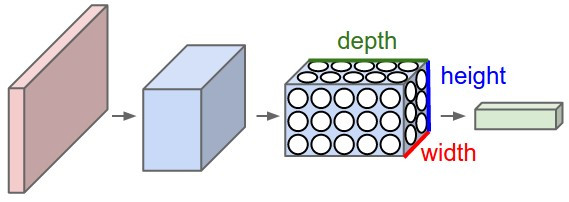
\includegraphics[width=0.8\textwidth]{./images/chapter3/cnn.jpg}
  \caption[Τρισδιάστατη κατανομή των νευρώνων στα CNN]{Τρισδιάστατη κατανομή των νευρώνων στα CNN}
  \label{fig:cnn_1}
\end{figure}

Κάθε επίπεδο ενός CNN παίρνει σαν είσοδο μία μορφή όγκου την οποία
και μετασχηματίζει σε μία άλλη μορφή όγκου.

Οι τρεις βασικοί τύποι επιπέδων που χρησιμοποιούνται σε αρχιτεκτονικές CNN είναι:
\begin{itemize}
  \item{Επίπεδο Συνέλιξης - Convolutional Layer (CONV)}
  \item{Επίπεδο Υπό-δειγματοληψίας- Pooling Layer (POOL)}
  \item{Πλήρη Συνδεδεμένο Επίπεδο - Fully-Connected Layer (FC)}
\end{itemize}
Μία σημαντική παρατήρηση είναι ότι τα επίπεδα CONV και FC έχουν παραμέτρους, δηλαδή
βάρη και τιμή πόλωσης των νευρώνων, ενώ τα επίπεδα POOL εκτελούν λειτουργία
δειγματοληψίας στα δεδομένα εισόδου τους.


\subsection{Επίπεδο Συνέλιξης}

Τα επίπεδα συνέλιξης είναι ο πυρήνας των μοντέλων CNN. Οι παράμετροι ενός
επιπέδου CONV είναι μία σειρά από δισδιάστατα φίλτρα τα οποία όμως εκτείνονται
σε όλο το σε όλο το βάθος του όγκου εισόδου. Το βάθος των φίλτρων αυτών
ισούται με το βάθος του όγκου στην είσοδο.


Όπως αναφέραμε και προηγουμένως, τα επίπεδα CONV εφαρμόζουν πράξη συνέλιξης πάνω στα
δεδομένα εισόδου. Αυτό επηρεάζει στην δομή των "τοπικών" διασυνδέσεων.
Στο παράδειγμα του σχήματος \ref{fig:cnn_2} βλέπουμε πως ο κάθε νευρώνας
του επιπέδου συνέλιξης συνδέεται με μία περιοχή του όγκου στην είσοδό του.

\begin{figure}[!ht]
  \centering
  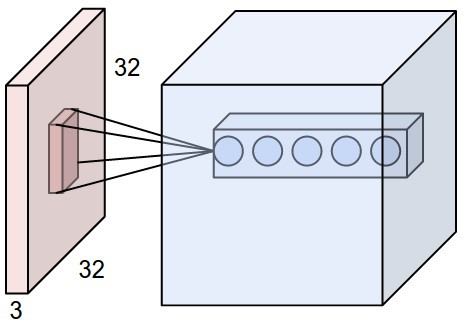
\includegraphics[width=0.4\textwidth]{./images/chapter3/cnn_2.jpg}
  \caption[%
    Παράδειγμα διασύνδεσης τρισδιάστατης εισόδου με την τρισδιάστατη δομή των
    νευρόνων ενός επιπέδου συνέλιξης (CONV)]{%
    Παράδειγμα διασύνδεσης τρισδιάστατης εισόδου με την τρισδιάστατη δομή των
    νευρόνων ενός επιπέδου συνέλιξης (CONV)}
  \label{fig:cnn_2}
\end{figure}

Η συνέλιξη ενός φίλτρου με τον τον όγκο εισόδου παράγει έναν \emph{χάρτη ενεργοποίησης (activation map)},
με τον τρόπο που φαίνεται στο \autoref{fig:cnn_activation_map}. Στο παράδειγμα αυτό
εφαρμόζεται φίλτρο διαστάσεων $5\times5\times3$ σε έναν όγκο $32\times32\times3$ και παράγεται
ένας χάρτης ενεργοποίησης διαστάσεων $28\times28\times1$.

\begin{figure}[!ht]
  \centering
  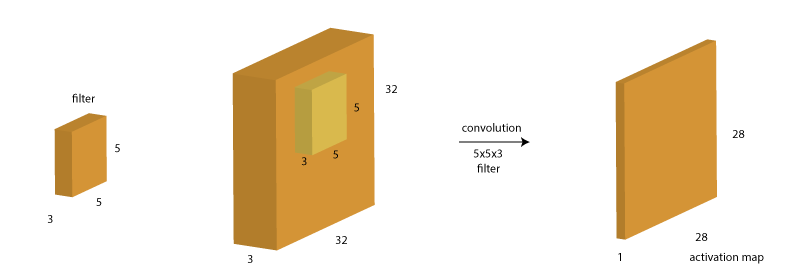
\includegraphics[width=1\textwidth]{./images/chapter3/cnn_activation_map.png}
  \caption[Συνέλιξη φίλτρου ενός επιπέδου συνέλιξης με τον όγκο εισόδου και παραγωγή ενός χάρτη ενεργοποίησης]{Συνέλιξη φίλτρου ενός επιπέδου συνέλιξης με τον όγκο εισόδου και παραγωγή ενός χάρτη ενεργοποίησης}
  \label{fig:cnn_activation_map}
\end{figure}

Η μείωση των διαστάσεων μήκους και πλάτους από $32\times32$ σε $28\times28$ οφείλεται στον τρόπο με τον οποίο
εκτελείται η πράξη της συνέλιξης των φίλτρων με τον όγκο εισόδου  (\autoref{fig:cnn_conv}).
Οι διαστάσεις του όγκου εξόδου, έχοντας σαν είσοδο όγκο διαστάσεων $N \times N \times d$ και φίλτρων $F \times F \times d$ υπολογίζονται, στην απλούστερη περίπτωση με βάση την σχέση
\begin{equation*}
  outsize = (N-F) + 1
\end{equation*}


\begin{figure}[!ht]
  \centering
  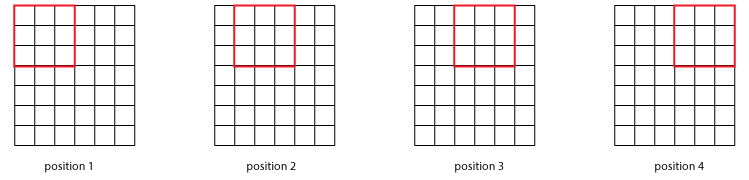
\includegraphics[width=1\textwidth]{./images/chapter3/cnn_conv.png}
  \caption[Διαδικασία Συνέλιξης]{Διαδικασία Συνέλιξης}
  \label{fig:cnn_conv}
\end{figure}

Η τιμή του βάθους του όγκου στην έξοδο ενός επιπέδου CONV αντιστοιχεί στον αριθμό των φίλτρων που
εφαρμόζονται στον όγκο εισόδου. Δηλαδή ο αριθμός των χαρτών ενεργοποίησης
αντιστοιχεί στον αριθμό των φίλτρων. Αν για παράδειγμα ο όγκος εισόδου είναι
διαστάσεων $32\times\32\times3$ και εφαρμόσουμε δέκα φίλτρα συνέλιξης διαστάσεων $5\times5\times3$,
ο όγκος εξόδου θα είναι διαστάσεων $28\times28\times3$ \autoref{fig:cnn_num_filters}.
Ο αριθμός των φίλτρων είναι μία παράμετρος, ή καλύτερα \emph{υπερ-παράμετρος} των επιπέδων συνέλιξης.

\begin{figure}[!ht]
  \centering
  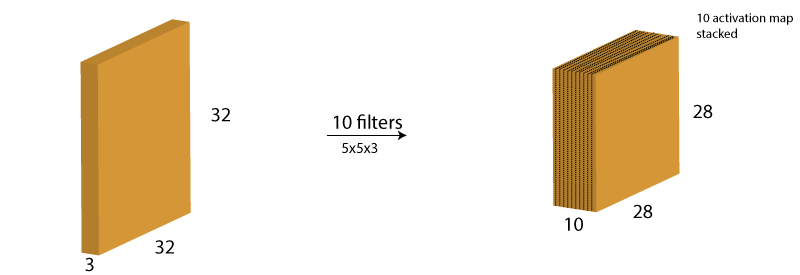
\includegraphics[width=1\textwidth]{./images/chapter3/cnn_num_filters.png}
  \caption[Αντιστοιχία του αριθμού των φίλτρων ενός επιπέδου συνέλιξης με το βάθος του όγκου στην έξοδο]{Αντιστοιχία του αριθμού των φίλτρων ενός επιπέδου συνέλιξης με το βάθος του όγκου στην έξοδο}
  \label{fig:cnn_num_filters}
\end{figure}

Ωστόσο, το βήμα μετατόπισης (stride) του φίλτρου πάνω στην είσοδο είναι και αυτό
μία υπέρ-παράμετρος (hyperparameter) των επιπέδων συνέλιξης.
Χρησιμοποιώντας βήμα μετατόπισης (S) διάφορο της μονάδας καταλήγουμε στην πιο κάτω
εξίσωση για τον υπολογισμό του όγκου εξόδου:
\begin{equation*}
  outsize = (N-F)/S + 1
\end{equation*}

Ένα πρόβλημα που εμφανίζεται στην περίπτωση των μοντέλων CNN με μεγάλο αριθμό
κρυφών επιπέδων είναι η γρήγορη μείωση των διαστάσεων μήκους και πλάτους του
όγκου, το οποίο είναι αποτέλεσμα της διαδοχική εφαρμογή πράξεων συνέλιξης (\autoref{fig:cnn_shrunk}).

\begin{figure}[!ht]
  \centering
  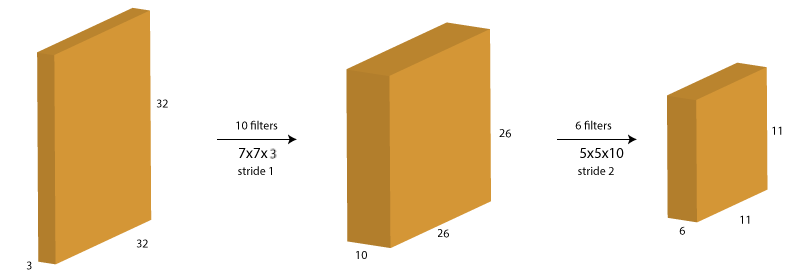
\includegraphics[width=1\textwidth]{./images/chapter3/cnn_shrunk.png}
  \caption[Διαδοχικές εφαρμογές του τελεστή συνέλιξης προκαλούν μείωση των διαστάσεων μήκους και πλάτους του όγκου]{Διαδοχικές εφαρμογές του τελεστή συνέλιξης προκαλούν μείωση των διαστάσεων μήκους και πλάτους του όγκου}
  \label{fig:cnn_shrunk}
\end{figure}

Αυτή η συμπεριφορά είναι ανεπιθύμητη αφού περιορίζει και τις διαστάσεις των φίλτρων
που μπορούμε να χρησιμοποιήσουμε σε κάθε επίπεδο CONV. Η χρήση φίλτρων μεγάλων
διαστάσεων φέρει σαν αποτέλεσμα την γρήγορη μείωση των διαστάσεων του όγκου.

Για να αποτρέψουμε αυτή την συμπεριφορά μπορούμε να επεκτείνουμε τις διαστάσεις
μήκους και πλάτους, προσθέτοντας μηδενικά στα σύνορα του όγκου εισόδου του
εκάστοτε επιπέδου CONV. Η διαδικασία αυτή ονομάζεται
\emph{zero-padding} και φαίνεται στο \autoref{fig:cnn_zero_padding}.
\begin{figure}[!ht]
  \centering
  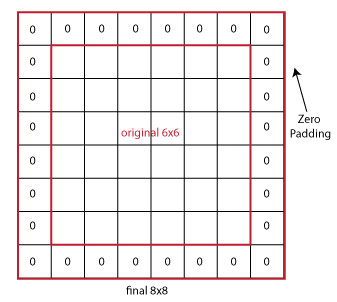
\includegraphics[width=0.6\textwidth]{./images/chapter3/cnn_zero_padding.png}
  \caption[Zero Padding]{Zero Padding}
  \label{fig:cnn_zero_padding}
\end{figure}
Το μέγεθος του συνόρου που προστίθεται είναι η τρίτη υπέρ-παράμετρος ενός
επιπέδου συνέλιξης.

Με την εισαγωγή της υπέρ-παραμέτρου zero-padding η εξίσωση υπολογισμού του όγκου
εξόδου έχει την μορφή:
\begin{equation*}
  outsize = (N - F + 2P)/S + 1
\end{equation*}

Συνοψίζοντας, ένα επίπεδο συνέλιξης έχει τα εξής χαρακτηριστικά:
\begin{itemize}
  \item{Διαστάσεις όγκου εισόδου: $W_{1} \times H_{1} \times D_{1}$}
  \item{Hyperparameters:}
    \begin{itemize}
      \item{K: Αριθμός φίλτρων}
      \item{F: Μέγεθος του φίλτρου ($F \times F$)}
      \item{S: Βήμα μετατόπισης}
      \item{P: Ποσότητα zero-padding}
    \end{itemize}
  \item{Διαστάσεις όγκου εξόδου: $W_{2} \times H_{2} \times D_{2}$, $D_{2} = K$} όπου:
    \begin{itemize}
      \item{$W_{2} = (W_{1} - F)/S + 1$}
      \item{$H_{2} = (H_{1} - F)/S + 1$}
      \item{$D_{2} = D_{1}$}
    \end{itemize}
\end{itemize}


\subsection{Επίπεδο Υπό-δειγματοληψίας - Pooling layer}

Συνήθως τα επίπεδα υπό-δειγματοληψίας προστίθενται στο δίκτυο, μεταξύ διαδοχικών
επιπέδων συνέλιξης. Η λειτουργία τους είναι να μειώσουν τις χωρικές
διαστάσεις των αναπαραστάσεων, μειώνοντας έτσι τον αριθμό των
παραμέτρων και άρα τους υπολογισμούς που γίνονται στο νευρωνικό δίκτυο
(\autoref{fig:cnn_pool}).

\begin{figure}[!ht]
  \centering
  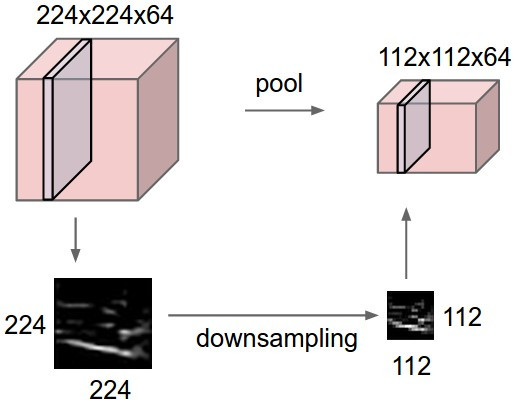
\includegraphics[width=0.6\textwidth]{./images/chapter3/cnn_pool.jpg}
  \caption[Επίπεδο Υποδειγματοληψίας - Pooling layer]{Επίπεδο Υπό-δειγματοληψίας - Pooling layer}
  \label{fig:cnn_pool}
\end{figure}
Ενεργεί δηλαδή σαν μία συνάρτηση υπό-δειγματοληψίας.
Πιθανές συναρτήσεις υπό-δειγματοληψίας είναι οι συναρτήσεις \emph{max, average και L2-Norm}

Στο \autoref{fig:cnn_pool_max} βλέπουμε το αποτέλεσμα της εφαρμογή της συνάρτησης
δειγματοληψίας $max(\vec{v})$ πάνω σε ένα πλέγμα διαστάσεων $4 \times 4$.

\begin{figure}[!ht]
  \centering
  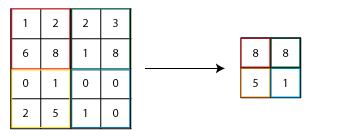
\includegraphics[width=0.6\textwidth]{./images/chapter3/cnn_pool_max.png}
  \caption[Συνάρτηση υπό-δειγματοληψίας Max - Max Pooling]{Συνάρτησης υποδειγματοληψίας Max - Max Pooling}
  \label{fig:cnn_pool_max}
\end{figure}

Τα χαρακτηριστικά των συναρτήσεων υπό-δειγματοληψίας είναι:
\begin{itemize}
  \item{Διαστάσεις όγκου εισόδου: $W_{1} \times H_{1} \times D_{1}$}
  \item{Hyperparameters:}
    \begin{itemize}
      \item{F: Χωρική τους έκταση ($F \times F$)}
      \item{S: Βήμα μετατόπισης}
    \end{itemize}
  \item{Διαστάσεις όγκου εξόδου: $W_{2} \times H_{2} \times D_{2}$, $D_{2} = K$} όπου:
    \begin{itemize}
      \item{$W_{2} = (W_{1} - F)/S + 1$}
      \item{$H_{2} = (H_{1} - F)/S + 1$}
      \item{$D_{2} = D_{1}$}
    \end{itemize}
\end{itemize}


\subsection{Πλήρως Συνδεδεμένο Επίπεδο - Fully-connected layer}

Ένα πλήρως συνδεδεμένο επίπεδο συνδέεται με όλους τους νευρώνες στο
προηγούμενο επίπεδο, όπως γίνεται στα απλά μοντέλα NN (Πολυεπίπεδος Perceptron),

Συνήθως το τελευταίο επίπεδο σε ένα CNN είναι πλήρως συνδεδεμένο και πιο
συγκεκριμένα έχει τόσους νευρώνες όσες και οι κλάσεις της πρόβλεψης. Για
παράδειγμα, ένα CNN που χρησιμοποιείται για αναγνώριση αντικειμένων σε
εικόνες CIFAR-10 έχει το τελευταίο επίπεδο του πλήρως συνδεδεμένο και
αποτελείται από 10 νευρώνες.


%\newevenside
\newevenside
\chapter{Τεχνικές Βαθιάς Μηχανικής Μάθησης και Αναγνώριση Αντικειμένωνν στον χώρο}
\label{chapter:theory}


\section{Deep Neural Networks}
\label{sec:theory_dnn}

The computations involved in producing an output from an input can be represented by a flow graph: a flow graph is a graph representing a computation, in which each node represents an elementary computation and a value (the result of the computation, applied to the values at the children of that node). Consider the set of computations allowed in each node and possible graph structures and this defines a family of functions. Input nodes have no children. Output nodes have no parents.

\section{Νευρωνικά Δίκτυα Συνέλιξης}
\label{sec:theory_cnn}

Μέχρι τώρα μιλήσαμε για τα πολυεπίπεδα νευρωνικά δίκτυα και την γενικότερη
λειτουργία τους. Σε αυτό το υποκεφάλαιο θα μιλήσουμε για συγκεκριμένα μοντέλα
πολυεπίπεδων νευρωνικών δικτύων και πιο συγκεκριμένα για τα
\emph{νευρωνικά Δίκτυα Συνέλιξης}. Τα συγκεκριμένα μοντέλα χρησιμοποιούνται
σήμερα κυρίως στα προβλήματα της αναγνώρισης και εντοπισμού αντικειμένων
σε εικόνες.

Ο τρόπος λειτουργίας τους είναι όμοιος με αυτόν που παρουσιάστηκε στο
\autoref{sec:dnn}; αποτελούνται από πολλά επίπεδα, όπου το κάθε επίπεδο αποτελείται
από έναν αριθμό νευρώνων οι οποίοι έχουν σαν παραμέτρους εκμάθησης τα βάρη ($w_{\jmath}^{\imath}$) τους
και την τιμή πόλωσης ($b^{\imath}$).
Κάθε νευρώνας δέχεται ένα σήμα εισόδου , εφαρμόζει μία πράξη εσωτερικού γινομένου σε αυτό,
και προαιρετικά περνάει το αποτέλεσμα από μία μη γραμμική συνάρτηση.
Το τελευταίο επίπεδο των CNN είναι ένας πλήρες συνδεδεμένο επίπεδο και έχει μία
συνάρτηση σφάλματος.
Η διαφορά των μοντέλων CNN από τα κλασσικά ANN είναι ότι θεωρούν για δεδομένα εισόδου
εικόνες.

Αυτό που καταφέρνουν να κάνουν τα CNN είναι να μοντελοποιήσουν μικρά
κομμάτια πληροφορίας τα οποία στην συνέχεια ενώνονται για να δημιουργήσουν
υψηλότερου επιπέδου πληροφορία. Αν για παράδειγμα παρατηρήσουμε την λειτουργία
ενός μοντέλου CNN, το πρώτο επίπεδο προσπαθεί να εντοπίσει ακμές, το δεύτερο
επίπεδο και παίρνοντας την πληροφορία αυτή των ακμών προσπαθεί να εντοπίσει περιγράμματα,
κτλ.


Σε κάθε πίξελ της εικόνας αντιστοιχούν 3 τιμές (RGB) και άρα η είσοδος σε ένα
CNN έχει τρεις διαστάσεις όπως φαίνεται και στο \autoref{fig:cnn_1}.
Για παράδειγμα ένα CNN το οποίο έχει σχεδιαστεί να δέχεται σαν είσοδο εικόνες ανάλυσης $80\times60$
έχει επίπεδο εισόδου διαστάσεων $80\times60\times3$.

\begin{figure}[!ht]
  \centering
  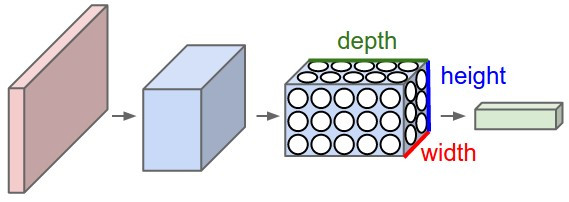
\includegraphics[width=0.8\textwidth]{./images/chapter3/cnn.jpg}
  \caption[Τρισδιάστατη κατανομή των νευρώνων στα CNN]{Τρισδιάστατη κατανομή των νευρώνων στα CNN}
  \label{fig:cnn_1}
\end{figure}

Κάθε επίπεδο ενός CNN παίρνει σαν είσοδο μία μορφή όγκου την οποία
και μετασχηματίζει σε μία άλλη μορφή όγκου.

Οι τρεις βασικοί τύποι επιπέδων που χρησιμοποιούνται σε αρχιτεκτονικές CNN είναι:
\begin{itemize}
  \item{Επίπεδο Συνέλιξης - Convolutional Layer (CONV)}
  \item{Επίπεδο Υπό-δειγματοληψίας- Pooling Layer (POOL)}
  \item{Πλήρη Συνδεδεμένο Επίπεδο - Fully-Connected Layer (FC)}
\end{itemize}
Μία σημαντική παρατήρηση είναι ότι τα επίπεδα CONV και FC έχουν παραμέτρους, δηλαδή
βάρη και τιμή πόλωσης των νευρώνων, ενώ τα επίπεδα POOL εκτελούν λειτουργία
δειγματοληψίας στα δεδομένα εισόδου τους.


\subsection{Επίπεδο Συνέλιξης}

Τα επίπεδα συνέλιξης είναι ο πυρήνας των μοντέλων CNN. Οι παράμετροι ενός
επιπέδου CONV είναι μία σειρά από δισδιάστατα φίλτρα τα οποία όμως εκτείνονται
σε όλο το σε όλο το βάθος του όγκου εισόδου. Το βάθος των φίλτρων αυτών
ισούται με το βάθος του όγκου στην είσοδο.


Όπως αναφέραμε και προηγουμένως, τα επίπεδα CONV εφαρμόζουν πράξη συνέλιξης πάνω στα
δεδομένα εισόδου. Αυτό επηρεάζει στην δομή των "τοπικών" διασυνδέσεων.
Στο παράδειγμα του σχήματος \ref{fig:cnn_2} βλέπουμε πως ο κάθε νευρώνας
του επιπέδου συνέλιξης συνδέεται με μία περιοχή του όγκου στην είσοδό του.

\begin{figure}[!ht]
  \centering
  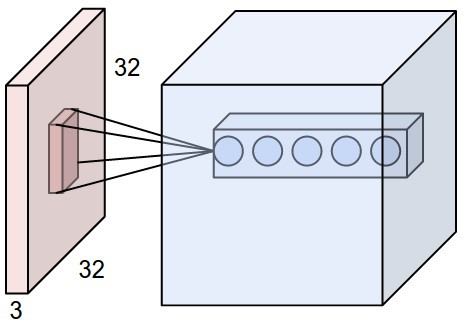
\includegraphics[width=0.4\textwidth]{./images/chapter3/cnn_2.jpg}
  \caption[%
    Παράδειγμα διασύνδεσης τρισδιάστατης εισόδου με την τρισδιάστατη δομή των
    νευρόνων ενός επιπέδου συνέλιξης (CONV)]{%
    Παράδειγμα διασύνδεσης τρισδιάστατης εισόδου με την τρισδιάστατη δομή των
    νευρόνων ενός επιπέδου συνέλιξης (CONV)}
  \label{fig:cnn_2}
\end{figure}

Η συνέλιξη ενός φίλτρου με τον τον όγκο εισόδου παράγει έναν \emph{χάρτη ενεργοποίησης (activation map)},
με τον τρόπο που φαίνεται στο \autoref{fig:cnn_activation_map}. Στο παράδειγμα αυτό
εφαρμόζεται φίλτρο διαστάσεων $5\times5\times3$ σε έναν όγκο $32\times32\times3$ και παράγεται
ένας χάρτης ενεργοποίησης διαστάσεων $28\times28\times1$.

\begin{figure}[!ht]
  \centering
  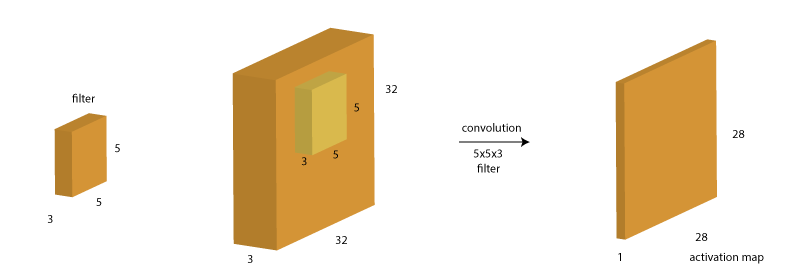
\includegraphics[width=1\textwidth]{./images/chapter3/cnn_activation_map.png}
  \caption[Συνέλιξη φίλτρου ενός επιπέδου συνέλιξης με τον όγκο εισόδου και παραγωγή ενός χάρτη ενεργοποίησης]{Συνέλιξη φίλτρου ενός επιπέδου συνέλιξης με τον όγκο εισόδου και παραγωγή ενός χάρτη ενεργοποίησης}
  \label{fig:cnn_activation_map}
\end{figure}

Η μείωση των διαστάσεων μήκους και πλάτους από $32\times32$ σε $28\times28$ οφείλεται στον τρόπο με τον οποίο
εκτελείται η πράξη της συνέλιξης των φίλτρων με τον όγκο εισόδου  (\autoref{fig:cnn_conv}).
Οι διαστάσεις του όγκου εξόδου, έχοντας σαν είσοδο όγκο διαστάσεων $N \times N \times d$ και φίλτρων $F \times F \times d$ υπολογίζονται, στην απλούστερη περίπτωση με βάση την σχέση
\begin{equation*}
  outsize = (N-F) + 1
\end{equation*}


\begin{figure}[!ht]
  \centering
  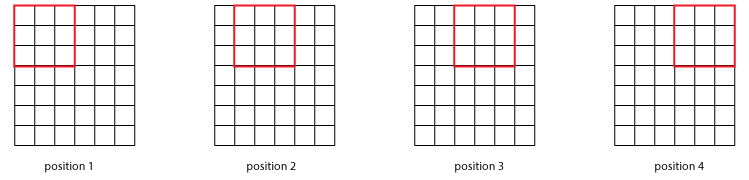
\includegraphics[width=1\textwidth]{./images/chapter3/cnn_conv.png}
  \caption[Διαδικασία Συνέλιξης]{Διαδικασία Συνέλιξης}
  \label{fig:cnn_conv}
\end{figure}

Η τιμή του βάθους του όγκου στην έξοδο ενός επιπέδου CONV αντιστοιχεί στον αριθμό των φίλτρων που
εφαρμόζονται στον όγκο εισόδου. Δηλαδή ο αριθμός των χαρτών ενεργοποίησης
αντιστοιχεί στον αριθμό των φίλτρων. Αν για παράδειγμα ο όγκος εισόδου είναι
διαστάσεων $32\times\32\times3$ και εφαρμόσουμε δέκα φίλτρα συνέλιξης διαστάσεων $5\times5\times3$,
ο όγκος εξόδου θα είναι διαστάσεων $28\times28\times3$ \autoref{fig:cnn_num_filters}.
Ο αριθμός των φίλτρων είναι μία παράμετρος, ή καλύτερα \emph{υπερ-παράμετρος} των επιπέδων συνέλιξης.

\begin{figure}[!ht]
  \centering
  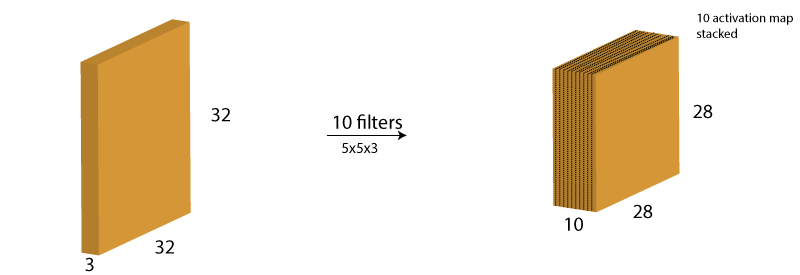
\includegraphics[width=1\textwidth]{./images/chapter3/cnn_num_filters.png}
  \caption[Αντιστοιχία του αριθμού των φίλτρων ενός επιπέδου συνέλιξης με το βάθος του όγκου στην έξοδο]{Αντιστοιχία του αριθμού των φίλτρων ενός επιπέδου συνέλιξης με το βάθος του όγκου στην έξοδο}
  \label{fig:cnn_num_filters}
\end{figure}

Ωστόσο, το βήμα μετατόπισης (stride) του φίλτρου πάνω στην είσοδο είναι και αυτό
μία υπέρ-παράμετρος (hyperparameter) των επιπέδων συνέλιξης.
Χρησιμοποιώντας βήμα μετατόπισης (S) διάφορο της μονάδας καταλήγουμε στην πιο κάτω
εξίσωση για τον υπολογισμό του όγκου εξόδου:
\begin{equation*}
  outsize = (N-F)/S + 1
\end{equation*}

Ένα πρόβλημα που εμφανίζεται στην περίπτωση των μοντέλων CNN με μεγάλο αριθμό
κρυφών επιπέδων είναι η γρήγορη μείωση των διαστάσεων μήκους και πλάτους του
όγκου, το οποίο είναι αποτέλεσμα της διαδοχική εφαρμογή πράξεων συνέλιξης (\autoref{fig:cnn_shrunk}).

\begin{figure}[!ht]
  \centering
  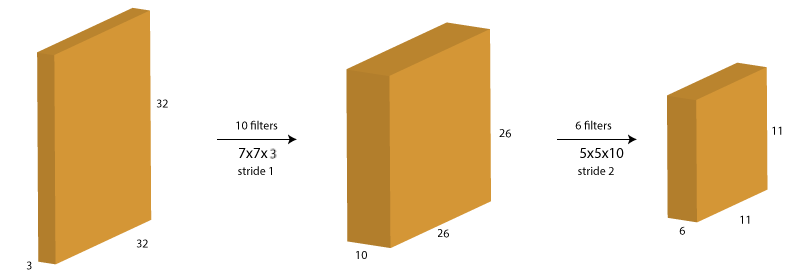
\includegraphics[width=1\textwidth]{./images/chapter3/cnn_shrunk.png}
  \caption[Διαδοχικές εφαρμογές του τελεστή συνέλιξης προκαλούν μείωση των διαστάσεων μήκους και πλάτους του όγκου]{Διαδοχικές εφαρμογές του τελεστή συνέλιξης προκαλούν μείωση των διαστάσεων μήκους και πλάτους του όγκου}
  \label{fig:cnn_shrunk}
\end{figure}

Αυτή η συμπεριφορά είναι ανεπιθύμητη αφού περιορίζει και τις διαστάσεις των φίλτρων
που μπορούμε να χρησιμοποιήσουμε σε κάθε επίπεδο CONV. Η χρήση φίλτρων μεγάλων
διαστάσεων φέρει σαν αποτέλεσμα την γρήγορη μείωση των διαστάσεων του όγκου.

Για να αποτρέψουμε αυτή την συμπεριφορά μπορούμε να επεκτείνουμε τις διαστάσεις
μήκους και πλάτους, προσθέτοντας μηδενικά στα σύνορα του όγκου εισόδου του
εκάστοτε επιπέδου CONV. Η διαδικασία αυτή ονομάζεται
\emph{zero-padding} και φαίνεται στο \autoref{fig:cnn_zero_padding}.
\begin{figure}[!ht]
  \centering
  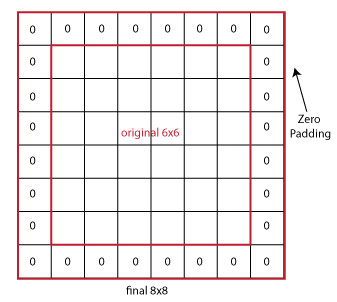
\includegraphics[width=0.6\textwidth]{./images/chapter3/cnn_zero_padding.png}
  \caption[Zero Padding]{Zero Padding}
  \label{fig:cnn_zero_padding}
\end{figure}
Το μέγεθος του συνόρου που προστίθεται είναι η τρίτη υπέρ-παράμετρος ενός
επιπέδου συνέλιξης.

Με την εισαγωγή της υπέρ-παραμέτρου zero-padding η εξίσωση υπολογισμού του όγκου
εξόδου έχει την μορφή:
\begin{equation*}
  outsize = (N - F + 2P)/S + 1
\end{equation*}

Συνοψίζοντας, ένα επίπεδο συνέλιξης έχει τα εξής χαρακτηριστικά:
\begin{itemize}
  \item{Διαστάσεις όγκου εισόδου: $W_{1} \times H_{1} \times D_{1}$}
  \item{Hyperparameters:}
    \begin{itemize}
      \item{K: Αριθμός φίλτρων}
      \item{F: Μέγεθος του φίλτρου ($F \times F$)}
      \item{S: Βήμα μετατόπισης}
      \item{P: Ποσότητα zero-padding}
    \end{itemize}
  \item{Διαστάσεις όγκου εξόδου: $W_{2} \times H_{2} \times D_{2}$, $D_{2} = K$} όπου:
    \begin{itemize}
      \item{$W_{2} = (W_{1} - F)/S + 1$}
      \item{$H_{2} = (H_{1} - F)/S + 1$}
      \item{$D_{2} = D_{1}$}
    \end{itemize}
\end{itemize}


\subsection{Επίπεδο Υπό-δειγματοληψίας - Pooling layer}

Συνήθως τα επίπεδα υπό-δειγματοληψίας προστίθενται στο δίκτυο, μεταξύ διαδοχικών
επιπέδων συνέλιξης. Η λειτουργία τους είναι να μειώσουν τις χωρικές
διαστάσεις των αναπαραστάσεων, μειώνοντας έτσι τον αριθμό των
παραμέτρων και άρα τους υπολογισμούς που γίνονται στο νευρωνικό δίκτυο
(\autoref{fig:cnn_pool}).

\begin{figure}[!ht]
  \centering
  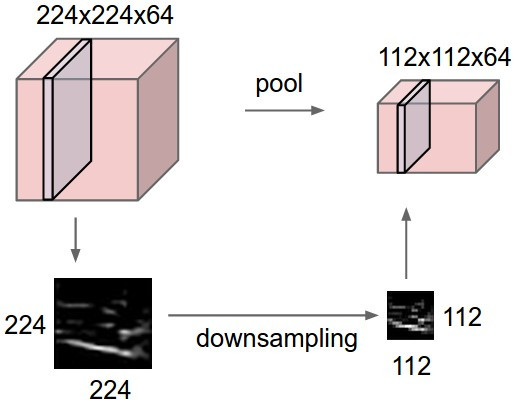
\includegraphics[width=0.6\textwidth]{./images/chapter3/cnn_pool.jpg}
  \caption[Επίπεδο Υποδειγματοληψίας - Pooling layer]{Επίπεδο Υπό-δειγματοληψίας - Pooling layer}
  \label{fig:cnn_pool}
\end{figure}
Ενεργεί δηλαδή σαν μία συνάρτηση υπό-δειγματοληψίας.
Πιθανές συναρτήσεις υπό-δειγματοληψίας είναι οι συναρτήσεις \emph{max, average και L2-Norm}

Στο \autoref{fig:cnn_pool_max} βλέπουμε το αποτέλεσμα της εφαρμογή της συνάρτησης
δειγματοληψίας $max(\vec{v})$ πάνω σε ένα πλέγμα διαστάσεων $4 \times 4$.

\begin{figure}[!ht]
  \centering
  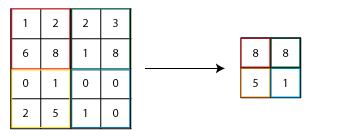
\includegraphics[width=0.6\textwidth]{./images/chapter3/cnn_pool_max.png}
  \caption[Συνάρτηση υπό-δειγματοληψίας Max - Max Pooling]{Συνάρτησης υποδειγματοληψίας Max - Max Pooling}
  \label{fig:cnn_pool_max}
\end{figure}

Τα χαρακτηριστικά των συναρτήσεων υπό-δειγματοληψίας είναι:
\begin{itemize}
  \item{Διαστάσεις όγκου εισόδου: $W_{1} \times H_{1} \times D_{1}$}
  \item{Hyperparameters:}
    \begin{itemize}
      \item{F: Χωρική τους έκταση ($F \times F$)}
      \item{S: Βήμα μετατόπισης}
    \end{itemize}
  \item{Διαστάσεις όγκου εξόδου: $W_{2} \times H_{2} \times D_{2}$, $D_{2} = K$} όπου:
    \begin{itemize}
      \item{$W_{2} = (W_{1} - F)/S + 1$}
      \item{$H_{2} = (H_{1} - F)/S + 1$}
      \item{$D_{2} = D_{1}$}
    \end{itemize}
\end{itemize}


\subsection{Πλήρως Συνδεδεμένο Επίπεδο - Fully-connected layer}

Ένα πλήρως συνδεδεμένο επίπεδο συνδέεται με όλους τους νευρώνες στο
προηγούμενο επίπεδο, όπως γίνεται στα απλά μοντέλα NN (Πολυεπίπεδος Perceptron),

Συνήθως το τελευταίο επίπεδο σε ένα CNN είναι πλήρως συνδεδεμένο και πιο
συγκεκριμένα έχει τόσους νευρώνες όσες και οι κλάσεις της πρόβλεψης. Για
παράδειγμα, ένα CNN που χρησιμοποιείται για αναγνώριση αντικειμένων σε
εικόνες CIFAR-10 έχει το τελευταίο επίπεδο του πλήρως συνδεδεμένο και
αποτελείται από 10 νευρώνες.


%\newevenside
\newevenside
\chapter{Εργαλεία Hardware/Software που χρησιμοποιήθηκαν}
\label{chapter:tools_hw_sw}

TODO Introduction!!


\section{NVIDIA Jetson TK1 development board}
\label{sec:jetson_tk1}

Στο κεφάλαιο αυτό παρουσιάζεται η ενσωματωμένη πλατφόρμα Jetson TK1 της NVIDIA,
η οποία χρησιμοποιήθηκε για εφαρμογή των υλοποιήσεων για
\emph{Αναγνώριση και Εντοπισμό Αντικειμένων} σε συστήματα πραγματικού χρόνου,
με Νευρωνικά Δίκτυα Συνέλιξης.

Ο \emph{Tegra K1} είναι το πρώτο SOC της NVIDIA, για φορητές συσκευές, με προηγμένη αρχιτεκτονική
και χαρακτηριστικά, καθώς και χαμηλή κατανάλωση ισχύως. H μέγιστη κατανάλωση είναι στα \emph{3Watt},
τιμή που δικαιολογεί την ενσωμάτωση του σε φορητές συσκευές (tablets, smartphones), καθώς και
σε προηγμένα ενσωματωμένα συστήματα (embedded systems) για εφαρμογές πραγματικού χρόνου.
\begin{figure}[H]
  \centering
  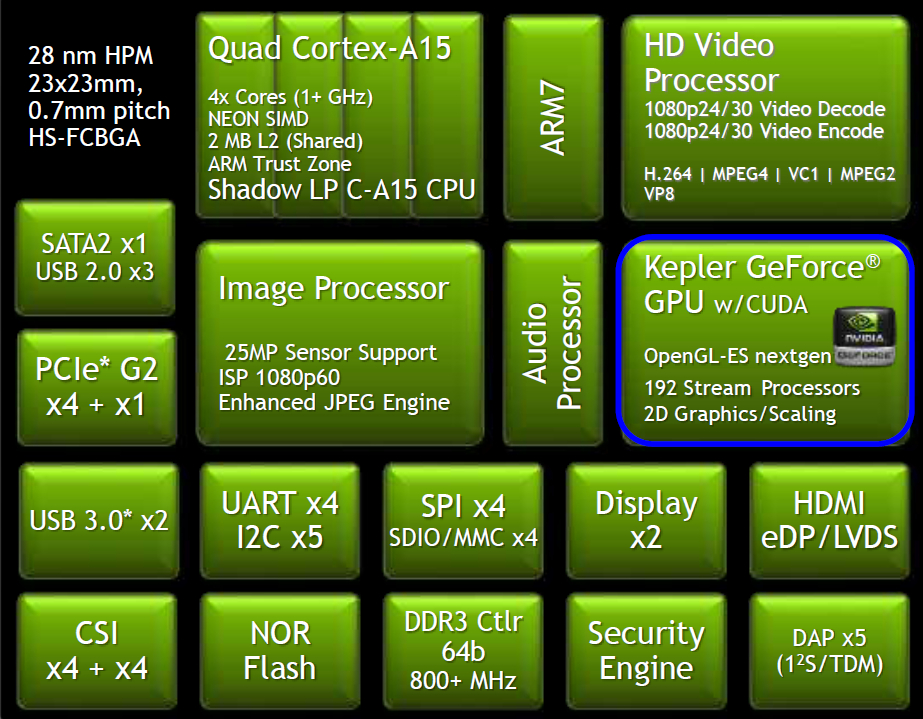
\includegraphics[width=0.7\textwidth]{./images/chapter4/nvidia_tegrak1_block2.jpg}
  \caption{Tegra K1 SOC}
  \label{fig:tegrak1soc}
\end{figure}
\noindent
Όπως φαίνεται στο \autoref{fig:tegrak1soc}, τα βασικά τεχνικά χαρακτηριστικά του Tegra K1 SOC:
\begin{itemize}
  \item{CPU: Quad-core ARM Cortex-A15 CPU, 2.3Ghz}
  \item{GPU: GK20A Kepler-based GPU with 192 CUDA cores}
  \item{RAM: DDR3L/LPDDR3, up to 8GB}
  \item{Peripherals I/O: USB, eMMC/SD-card, LVDS, HDMI, SPI, UART, I2C, SATA, PCIe}
  \item{ISP: Image processor}
\end{itemize}

Στα πλαίσια της παρούσας διπλωματικής εργασίας, επιλέκτηκε να χρησιμοποιή-σουμε το
\emph{Jetson TK1} development board της NVIDIA, που φαίνετaι στο \autoref{fig:jetson_tk1}.
\begin{figure}[!ht]
  \centering
  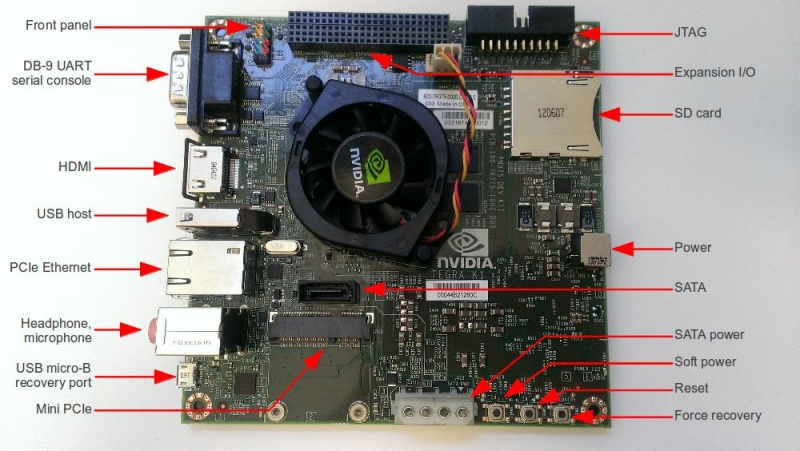
\includegraphics[width=0.9\textwidth]{./images/chapter4/jetson-tk1-labelled.jpg}
  \caption[Jetson TK1 development board]{Jetson TK1 development board}
  \label{fig:jetson_tk1}
\end{figure}
Το Jetson TK1 ενσωματώνει το Tegra K1 SOC (CPU+GPU+ISP)
και είναι πλήρες συμβατό με διάφορες διανομές λειτουργικών συστημάτων Linux (Ubuntu, Debian, Arch, Fedora, openSUSE, Gentoo).
Η πλήρης συμβατότητα και υποστήριξη λειτουργικού συστήματος Linux ήταν βασικό κριτήριο
στην επιλογή του συγκεκριμένου ενσωματωμένου συστήματος αφού επιτρέπει την
εγκατάσταση εργαλείων με τον ίδιο τρόπο όπως σε ένα σταθερό υπολογιστικό σύστημα (Desktop PC)
το οποίο τρέχει Linux OS. Πέρα από την συμβατότητα με κλασσικές διανομές Linux OS,
η NVIDIA έχει αναπτύξει δικό της λειτουργικό σύστημα, \emph{Linux4Tegra}, το οποίο
έχει σαν βάση τα Ubuntu-14.04, με κάποιες επεκτάσεις για πλήρη υποστήριξη του hardware του Jetson TK1.
Επιπλέον παράγοντας στην επιλογή της συγκεκριμένης πλατφόρμας είναι η πληθώρα των περιφερειακων διεπαφών που
διαθέτει, κάνοντας το χρήσιμο για εφαρμογή σε ρομποτικά συστήματα όπου η σύνδεση διαφόρων περιφεριακών συσκευών,
όπως για παράδειγμα αισθητήρες, κάμερες, κινητήρες, σερβο-κινητήρες, είναι απαίτηση.
Πιο κάτω δίνονται οι βασικές διεπαφές που προσφέρει η πλατφόρμα Jetson TK1:
\begin{itemize}
  \setlength\itemsep{0em}
  \item{mini-PCIe: Σύνδεση πρόσθετων συσκευών στον δίαυλο PCI-Express όπως, Wifi cards, SSD δίσκων, κτλ.}
  \item{USB 2.0 port: Για σύνδεση συσκευών ή/και αισθητήρων με διεπαφή eHCI (Extended Host Controller Interface)}
  \item{USB 3.0 port: Για σύνδεση συσκευών ή/και αισθητήρων με διεπαφή xHCI (eXtensible Host Controller Interface)}
  \item{HDMI: Δίνει την δυνατότητα σύνδεσης οθόνης}
  \item{RS232 port: Παρόλο που το RS232 είναι αρκετά παλιό προτόκολο επκοινωνίας, ακόμη ενσωματώνεται σε διάφορες συσκευές που δεν απαιτούν μεγάλο όγκο μεταφοράς δεδομένων, όπως οι οδηγοί κινητήρων}
  \item{Audio IO}
  \item{Gigabit Ethernet LAN: Δικτύωση της πλατφόρμας με τον "έξω" κόσμο}
  \item{SATA: Επιτρέπει την σύνδεση σκληρού δίσκου SATA}
  \item{JTAG port: Το JTAG προσφέρει την δυνατότητα σύνδεσης συσκευής/προγράμματος εντοπισμού σφαλμάτων (debugger), για επαγγελματική αποσφαλμάτωση}
  \item{UART port}
  \item{I2C ports: Διαθέτει τρείς θύρες I2C για σύνδεση αισθητήρων/συσκευών που οδηγούνται με το συγκεκριμένο προτόκολο}
  \item{GPIO: Προσφέρει δύο θυρες επέκτασης (expansion ports), με 50 και 75 ακροδέκτες αντίστοιχα. Χρησιμο κυρίως για, επικοινωνία συσκευών με SPI, οδήγηση σερβο-κινητήρων, διακλάδωση τροφοδοσίας σε τρίτες συσκευές, κτλ.}
\end{itemize}

Όσον αφορά την υλοποίηση και ανάπτυξη Νευρωνικών Δικτύων σε ενσωματωμένα συστήματα,
η πλατφόρμα Jetson TK1 θεωρείτε ιδανική αφού υποστηρίζει CUDA και cuDNN.
H cuDNN (CUDA Deep Neural Network library) είναι GPU-accelerated βιβλιοθήκη για Νευρωνικά Δίκτυα,
η οποία αναπτύχθηκε από την NVIDIA και προσφέρει υψηλού επιπέδου υλοποιήσεις για ρουτίνες όπως συνέλιξη, κανονικοποίηση δεδομένων, pooling, επίπεδα ενεργοποίησης, κτλ.
Η βιβλιοθήκη cuDNN χρησιμοποιέιτε και ενσωματώνεται στα πιο δημοφιλή σήμερα frameworks για σχεδίαση και υλοποίηση μοντέλων DNN,
όπως Caffe \cite{jia2014caffe}, Tensorflow \cite{DBLP:journals/corr/AbadiBCCDDDGIIK16},
Theano \cite{2016arXiv160502688full}\cite{bergstra+al:2010-scipy}\cite{Bastien-Theano-2012},
Torch \cite{collobert2002torch}\cite{collobert2011torch7}\cite{collobert2012implementing}, CNTΚ και Keras.

\begin{figure}[!ht]
  \centering
  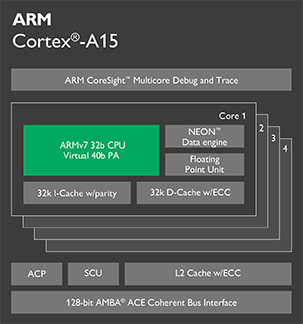
\includegraphics[width=0.6\textwidth]{./images/chapter4/cortex_A15_chip_diagram.png}
  \caption[Jetson TK1 development board]{Jetson TK1 development board}
  \label{fig:cortex_A15}
\end{figure}

Ένα από τα μειονεκτήματα της πλατφόρμας Jetson TK1 είναι αρχιτεκτονική των 32 bit του επεξεργαστή ARM Cortex-A15 MPCore
που έχει ενσωματωμένοv \autoref{fig:cortex_A15}. Με την εμφάνιση των επεξεργαστών ARM Cortex-A57, οι οποίοι είναι αρχιτεκτονικής 64 bit,
η υποστήριξη σε λογισμικά, τόσο από την πλευρά της NVIDIA όσο και από την ανοικτού-κώδικα (open-source) κοινότητα, μειώθηκε.
Η NVIDIA σταμάτησε να υποστηρίζει μηχανήματα αρχιτεκτονικής 32 bit, τις βιβλιοθήκες CUDA και cuDNN,
από την έκτη και δεύτερη έκδοση αντίστοιχα. Η CUDA είναι σήμερα στην έκδοση 8 και η cuDNN στην έκδοση 5,
οι οποίες φέρουν τρομερές αλλαγές στην επίδοση των αλγορίθμων βαθιάς εκμάθησης
(\href{https:/developer/nvidia/cudnn}{https:/developer/nvidia/cudnn}).

\section{Εργαλεία Λογισμικού}
\label{sec:dnn_sw}

Λόγω της ραγδαίας εξέλιξης της επιστήμης της βαθιάς μηχανικής μάθησης,
έχουν αναπτυχθεί τα τελευταία χρόνια και πολλά εργαλεία λογισμικού (βιβλιοθήκες, SDKs, frameworks)
για γρήγορη ή/και αποτελεσματική σχεδίαση και υλοποίηση πολυεπίπεδων νευρωνικών δικτύων.

Θωρούμε σημαντικό να αναφέρουμε σε αυτό το σημείο μερικά από τα πιο γνωστά εργαλεία
σχεδίασης και ανάπτυξης αλγορίθμων και μοντέλων πολυεπίπεδων νευρωνικών δικτύων, τα οποία
και χρησιμοποιούνται από την επιστημονική κοινότητα:
\begin{itemize}
  \item{Caffe \footnote{\href{http://caffe.berkeleyvision.org/}{http://caffe.berkeleyvision.org/}} %
      \cite{jia2014caffe}:
    Framework για σχεδίαση υλοποίηση και δοκιμή μοντέλων βαθιάς μηχανικής μάθησης.
    Είναι ένα από τα πρώτα ανοικτού κώδικα εργαλεία βαθιάς μηχανικής μάθησης που αναπτύχθηκαν.}
  \item{Tensorflow \footnote{\href{https://www.tensorflow.org/}{https://www.tensorflow.org/}} %
      \cite{DBLP:journals/corr/AbadiBCCDDDGIIK16}:
    Ανοικτού κώδικα βιβλιοθήκη για αριθμητικούς υπολογισμούς χρησιμοποιώντας
    γράφους ροής δεδομένων ανεπτυγμένο από την ερευνητική ομάδα της Google.
    Η ευέλικτη αρχιτεκτονική της επιτρέπει την ανάπτυξη
    λογισμικού σε μία ή και περισσότερες κεντρικές μονάδες επεξεργασίας CPU ή μονάδες GPU.}
  \item{Theano \footnote{\href{http://deeplearning.net/software/theano/}{http://deeplearning.net/software/theano/}}
      \cite{2016arXiv160502688full}\cite{bergstra+al:2010-scipy}\cite{Bastien-Theano-2012}: %
      Βιβλιοθήκη για Python η οποία επιτρέπει τον ορισμό, βελτιστοποίηση και αξιολόγηση
      μαθηματικών συναρτήσεων που αφορούν πράξεις με πολυδιάστατους πίνακες.}
      %Τα βασικά χαρακτηριστικά της είναι:}
    %\begin{itemize}
      %\item{Ανοικτού κώδικα}
      %\item{Ενσωματώνει την βιβλιοθήκη NumPy \footnote{http://www.numpy.org/}}
    %\end{itemize}
    \item{Torch \footnote{\href{http://torch.ch/}{http://torch.ch/}} %
        \cite{collobert2002torch}\cite{collobert2011torch7}\cite{collobert2012implementing}:
      Framework για γρήγορη ανάπτυξη και δοκιμή αλγορίθμων μηχανικής μάθησης.}
    \item{Keras \footnote{\href{https://keras.io/}{https://keras.io/}} \cite{chollet2015keras}:
    Ανοικτού κώδικα, υψηλού επιπέδου βιβλιοθήκη σε Python για σχεδίαση και ανάπτυξη
    πολυεπίπεδων νευρωνικών δικτύων. Ενσωματώνει
    τις βιβλιοθήκες Theano και Tensorflow και προσφέρει.}
  \item{CNTK \footnote{\href{https://www.cntk.ai/}{https://www.cntk.ai/}} \cite{Seide:2016:CMO:2939672.2945397}:
    Σετ από εργαλεία για εφαρμογές βαθιάς μηχανικής μάθησης, ανεπτυγμένο από την ερευνητική ομάδα της Microsoft.}
\end{itemize}

Μία σημαντική παρατήρηση είναι ότι όλα τα προαναφερθέντα εργαλεία χρησιμοποιούν μοντέλα γράφων
για την συμβολική αναπαράσταση των μαθηματικών υπολογισμών. Η αναπαράσταση σε μορφή γράφων
έχει αποδειχθεί αποτελεσματική όσον αφορά την ταχύτητα υπολογισμών μαθηματικών εκφράσεων, αλλά και την
απλότητα ανάπτυξης \autoref{fig:graph_model_example}.

\begin{figure}[!ht]
  \centering
  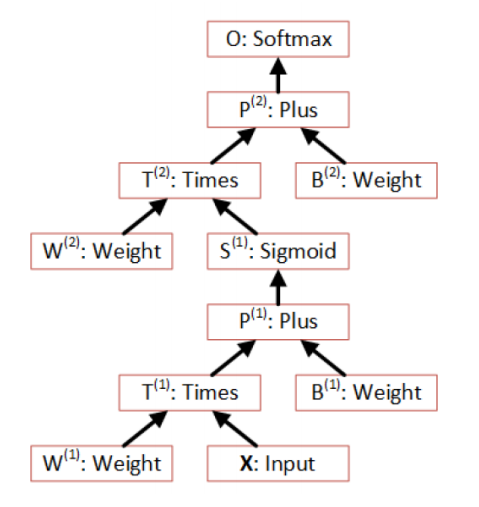
\includegraphics[width=0.6\textwidth]{./images/chapter4/graph_model_example.png}
  \caption[Παράδειγμα αναπαράστασης ενός μοντέλου νευρωνικού δικτύου σε γράφο.
    Το ΝΝ αποτλείται από ένα κρυφό επίπεδο
    και ένα ταξινομητή Sotfmax στο επίπεδο εξόδου]{
    Παράδειγμα αναπαράστασης ενός μοντέλου νευρωνικού δικτύου σε γράφο.
    Το ΝΝ απειλείται από ένα κρυφό επίπεδο με συνάρτηση ενεργοποίησης την σιγμοειδή συνάρτηση
    και έναν ταξινομητή Sotfmax στο επίπεδο εξόδου}
  \label{fig:graph_model_example}
\end{figure}
Οι κόμβοι στον γράφο αναπαριστούν μαθηματικές πράξεις ή εκφράσεις, ενώ τα φύλλα
αναπαριστούν πολυδιάστατους πίνακες δεδομένων, οι οποίοι ονομάζονται Tensors.

Καταλαβαίνουμε ότι η αναπαράσταση των νευρωνικών δικτύων σε μορφή γράφου ροής
δεδομένων προσθέτει ένα επίπεδο ευελιξίας στην ανάπτυξη τους. Μία σημαντική παρατήρηση
είναι ότι ο γράφος μπορεί χωριστεί σε πιο μικρούς γράφους και άρα να διανεμηθεί
σε περισσότερες από μία υπολογιστικές μονάδες (CPUs / GPUs) ή ακόμα και
σε ετερογενή διανεμημένα συστήματα (CPUs + GPUs) \cite{DBLP:journals/corr/AbadiABBCCCDDDG16} .

Ένα ακόμη αξιοσημείωτο εργαλείο είναι η βιβλιοθήκη \emph{ConvNetJS} \cite{karpathy2014convnetjs},
η οποία αναπτύχθηκε από τον Andrej Karpathy και τρέχει κατευθείαν σε σύγχρονους
Web Browsers
\footnote{Στον ιστοχώρο \href{http://cs.stanford.edu/people/karpathy/convnetjs/}{http://cs.stanford.edu/people/karpathy/convnetjs/}
υπάρχουν παραδείγματα μοντέλων νευρωνικών δικτύων τα οποία μπορεί ο αναγνώστης να δοκιμάσει
κατευθείαν μέσα από τον browser του}
ή/και σε υπολογιστικά συστήματα
\footnote{Η βιβλιοθήκη ConvNetJS μπορεί να τρέξει σε συστήματα τα οποία
υποστηρίζουν Node.js (server-side javascript interpreter)}.

Στα πλαίσια της παρούσας διπλωματικής εργασίας επιλέξαμε να χρησιμοποιήσουμε
την βιβλιοθήκη \emph{Keras} για τους εξής λόγους:
\begin{itemize}
  \item{Προσφέρει υψηλού επιπέδου ρουτίνες για ανάπτυξη νευρωνικών δικτύων}
  \item{Εύκολη και γρήγορη σχεδίαση και ανάπτυξη}
  \item{Υποστηρίζει Νευρωνικά Δίκτυα Συνέλιξης}
  \item{Παρέχει πολλά παραδείγματα σχεδίασης και ανάπτυξης}
  \item{Τρέχει αδιάλειπτα σε CPU και GPU}
  \item{Επιτρέπει την επιλογή μεταξύ των βιβλιοθηκών Theano και  Tensorflow
    για την εκτέλεση των μαθηματικών εκφράσεων}
\end{itemize}

Το τελευταίο είναι σημαντικό αφού μας επιτρέπει να αναπτύξουμε μοντέλα
και στην συνέχεια να αξιολογήσουμε την απόδοσή τους, κυρίως σε χρόνο εκτέλεσης,
με χρήση τόσο του Theano αλλά και Tensorflow, χωρίς να χρειαστεί
επαναπρογραμματισμός.




\newevenside
\chapter{Υλοποιήσεις}
\label{chapter:implementations}

Η παρούσα διπλωματική εργασία καταπιάνεται με το
πρόβλημα της ανάπτυξης νευρωνικών δικτύων στην πλατφόρμα Jetson TK1
και στοχεύει στην ανάπτυξη ενός νευρωνικού δικτύου για ταυτόχρονη
αναγνώριση και εντοπισμό αντικειμένων (object detection) σε εικόνες.

Ένα CNN αποτελείται από πολλά επίπεδα συνέλιξης, τα οποία με την σειρά τους
αποτελούνται από εκατομμύρια νευρώνες το κάθε ένα. Αυτό σημαίνει και εκατομμύρια
παραμέτρους όπου η καθεμία είναι ένας αριθμός κινητής υποδιαστολής 32 bit.
Το ενσωματωμένο σύστημα Jetson TK1 έχει περιορισμένη χωρητικότητα μνήμης (2GB),
γεγονός που λήφθηκε υπόψη κατά την επιλογή των μοντέλων CNN που υλοποιήθηκαν.

Οι υλοποιήσεις χωρίζονται σε 2 μέρη:
\begin{itemize}
  \item{Ανάπτυξη διαφόρων μοντέλων CNN για αναγνώριση αντικειμένων σε εικόνες}
  \item{Ρυθμίσεις και βελτιστοποιήσεις στο Jetson TK1}
\end{itemize}

Στο πρώτο μέρος παρουσιάζονται και αναλύονται τα μοντέλα CNN που αναπτύχθηκαν, ενώ στο
δεύτερο δίνεται μία πλήρης περιγραφή των διαδικασιών ρύθμισης και βελτιστοποίησης που έγιναν
στο ενσωματωμένο σύστημα Jetson TK1 καθώς και τα εργαλεία που χρειάστηκε να εγκατασταθούν.

\section{Μοντέλα CNN}
\label{sec:cnn_impl}

Όπως αναφέραμε \autoref{sec:dnn_sw} το βασικό εργαλείο λογισμικού που
χρησιμοποιήσαμε για την ανάπτυξη των μοντέλων CNN είναι το \emph{Keras}.

Η βιβλιοθήκη Keras προσφέρει τις υλοποιήσεις όλων των επιπέδων που
απαιτούνται για για την ανάπτυξη ενός CNN
\footnote{Πλήρες περιγραφή της λίστας των διαθέσιμων επιπέδων: \href{https://keras.io/layers/core/}{https://keras.io/layers/core/}}.
Πιο συγκεκριμένα, τα επίπεδα που χρησιμοποιήθηκαν, καθώς και οι βασικές
παράμετροι τους περιγράφονται πιο κάτω:
\begin{itemize}
  \item{\textbf{InputLayer}: Επίπεδο Εισόδου του νευρωνικού δικτύου}
    \begin{itemize}
      \item{Διαστάσεις του όγκου εισόδου (tensor shape)}
    \end{itemize}
  \item{Convolution2D: Επίπεδο Συνέλιξης}
    \begin{itemize}
      \item{Μορφολογία της εισόδου}
      \item{Αριθμός των φίλτρων συνέλιξης}
      \item{Διαστάσεις των φίλτρων συνέλιξης}
      \item{Συνάρτηση ενεργοποίησης}
    \end{itemize}
  \item{MaxPooing2D: Επίπεδο Υποδειγματοληψίας}
    \begin{itemize}
      \item{Διαστάσεις πλαισίου}
      \item{Βήμα μετατόπισης}
    \end{itemize}
  \item{ZeroPadding2D: Προσθέτει πλαίσιο με μηδενικά στον όγκο εισόδου}
    \begin{itemize}
      \item{Διαστάσεις του πλαισίου}
    \end{itemize}
  \item{Activation: Επίπεδο ενεργοποίησης. Εφαρμόζει συνάρτηση ενεργοποίησης στον
    όγκο εξόδου του προηγούμενου επιπέδου}
  \item{Dropout: Επίπεδο πρόληψης υπέρ-προσαρμογής \cite{lecun2015deep}}
  \item{Dense: Πλήρες συνδεδεμένο επίπεδο}
    \begin{itemize}
      \item{Διαστάσεις του όγκου εισόδου (Προαιρετικό)}
      \item{Διαστάσεις του όγκου εξόδου}
      \item{Συνάρτηση ενεργοποίησης}
    \end{itemize}
  \item{Flatten: Μετασχηματίζει τον όγκου εισόδου σε επίπεδη αναπαράσταση
    (π.χ. για όγκο εισόδου $64 \times 32 \times 32$ η έξοδος θα είναι επίπεδη με $65536$ νευρώνες}
  \item{BatchNormalization: Εφαρμόζει μετασχηματισμό για να κρατήσει την μέση τιμή
      και την τυπική απόκλιση των ενεργοποιήσεων του προηγούμενου επιπέδου στις τιμές 0 και 1 αντίστοιχα}
\end{itemize}

Σημαντική παρατήρηση είναι το γεγονός ότι η επιστήμη της βαθιάς μηχανικής μάθησης
βρίσκεται σε πρώιμο στάδιο, με αποτέλεσμα να μην υπάρχουν συγκεντρωμένες
οι υλοποιήσεις των διαφόρων επιπέδων και γενικότερα των μοντέλων σύγχρονων ΑNN.

Περαιτέρω, η επιλογή των μοντέλων CNN για ανάπτυξη στηρίχθηκε στην ύπαρξη και
προ-εκπαιδευμένων βαρών για τα αντίστοιχα CNN στο διαδίκτυο για 2 λόγους:
\begin{itemize}
  \item{Η διαδικασία εκπαίδευσης είναι χρονοβόρα διαδικασία και προϋποθέτει
    τη χρησιμοποίηση μίας ή περισσοτέρων ισχυρών μονάδων GPU (NVIDIA Titam X GPU)}
  \item{Η εκπαίδευση νευρωνικών δικτύων ξεφεύγει από τα πλαίσια της παρούσας
    διπλωματικής εργασίας}
\end{itemize}


\subsection{AlexNet}

Το δίκτυο AlexNet ήταν η αρχή της εισαγωγής της βαθιάς
μηχανικής μάθησης στην επιστήμη της μηχανικής όρασης. Εμφανίστηκε και χρησιμοποιήθηκε
στον διαγωνισμό ImageNet ILSVRC challenge, το 2012, κερδίζοντας με διαφορά
10,9\%, στο σφάλμα αναγνώρισης αντικειμένων σε σύνολο 1000 κλάσεων.

\begin{figure}[!ht]
  \centering
  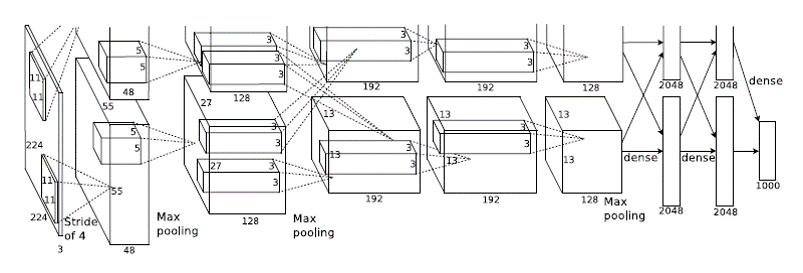
\includegraphics[width=1\textwidth]{./images/chapter5/alexnet_from_paper.png}
  \caption[Μοντέλο δικτύου AlexNet]{%
    Μοντέλο δικτύου AlexNet \\
    Πηγή: Άρθρο δημοσίευσης \emph{ImageNet Classification with Deep Convolutional Neural Networks} \cite{NIPS2012_4824}
  }
  \label{fig:alexnet_from_paper}
\end{figure}

Το συγκεκριμένο νευρωνικό δίκτυο συνέλιξης αποτελείται από σύνολο οκτώ επίπεδα,
ή καλύτερα ομάδες επιπέδων; πέντε επίπεδα συνέλιξης και 3 πλήρως συνδεδεμένα. \\

\begin{tabular}{ | l | l | l | l | }
  \hline
  \rowcolor{Gray}
  Επίπεδο  & Τύπος & Αριθμός καναλιών & Διαστάσεις φίλτρων \\
  \hline
  1 & Conv+Pool+Norm & 96 & $11 \times 11$ \\
  2 & Conv+Pool+Norm & 256 & $5 \times 5$ \\
  3 & Conv & 384 & $3 \times 3$ \\
  4 & Conv & 384 & $3 \times 3$ \\
  5 & Conv+Pool & 256 & $3 \times 3$ \\
  6 & Full & 4096 & Ν/A \\
  7 & Full & 4096 & N/A \\
  8 & Full & 1000 & N/A \\
  \hline
\end{tabular}
\\

Η συνάρτηση υποδειγματοληψίας που χρησιμοποιεί το μοντέλο είναι η συνάρτηση
MaxPooling2D με βήμα μετατόπισης ίσο με την μονάδα και στους 2 άξονες ($1 \times 1$).
Σε όλα τα επίπεδα εκτός του τελευταίου χρησιμοποιήθηκε η συνάρτηση ενεργοποίησης
ReLU. Επίσης χρησιμοποιεί και πολλά επίπεδα ZeroPadding με πλαίσιο
διαστάσεων $1 \times 1$. Το τελευταίο επίπεδο παίζει τον ρόλο του ταξινομητή και συγκεκριμένα
είναι ένας ταξινομητής Softmax.

Η υλοποίηση στηρίχτηκε στην αντίστοιχη που υπάρχει με το εργαλείο Caffe
\footnote{Υλοποίηση του δικτύου AlexNet στο Caffe: \url{https://github.com/BVLC/caffe/tree/master/models/bvlc_alexnet}}.
Πρακτικά μεταφράστηκε ο πηγαίος κώδικας της υλοποίησης από το Caffe στο Keras.
Ο αντίστοιχος γράφος της υλοποίησης του μοντέλου
φαίνεται φαίνεται στο \autoref{fig:alexnet_2}.

\begin{figure}[!ht]
  \centering
  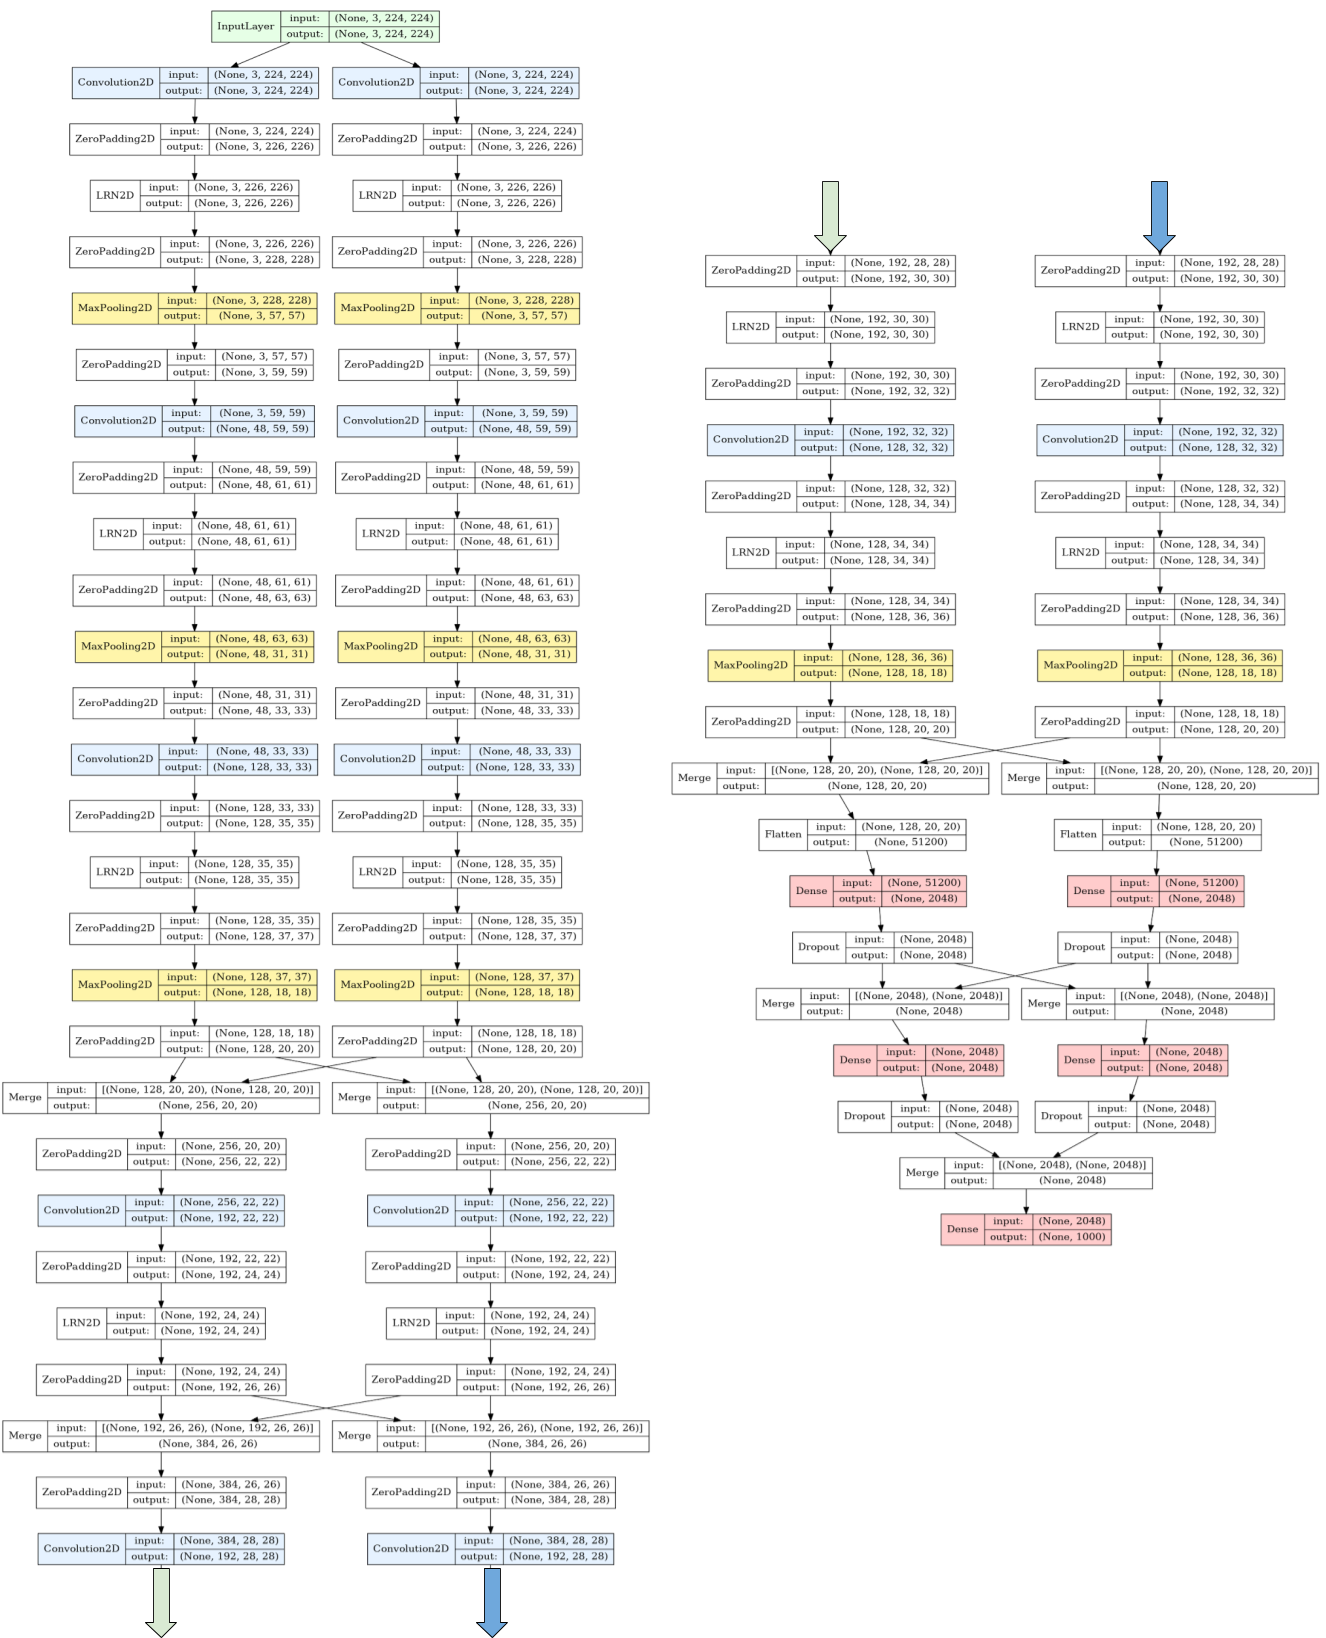
\includegraphics[width=1\textwidth]{./images/chapter5/alexnet_3.png}
  \caption[Πλήρες μορφή του δικτύου AlexNet της υλοποίησης]{Πλήρες μορφή του δικτύου AlexNet της υλοποίησης}
  \label{fig:alexnet_2}
\end{figure}

Το AlexNet είναι ένα μοντέλο μόνο για αναγνώριση και όχι για εντοπισμό
των αντικειμένων, δηλαδή η μόνη πληροφορία που μας δίνει είναι η κλάση των
αντικειμένων.

%% --------------------------------------------------------------------------
\subsection{VGG16}

Το δίκτυο VGG16 ήταν ο νικητής του διαγωνισμού ImageNet ILSVRC-2014 με σφάλμα
κατηγοριοποίησης 7.5\% σε σύνολο 1000 κλάσεων αντικειμένων \cite{Simonyan14c}.

\begin{figure}[!ht]
  \centering
  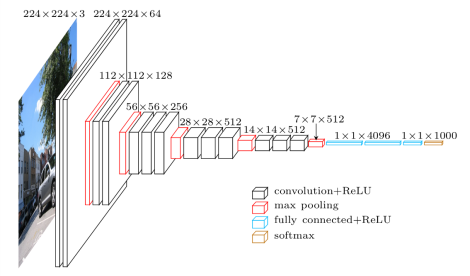
\includegraphics[width=0.8\textwidth]{./images/chapter5/vgg16_from_paper.png}
  \caption[Mορφή του δικτύου VGG16]{Μορφή του δικτύου VGG16}
  \label{fig:vgg16_from_paper}
\end{figure}

Αποτελείτε από 16 επίπεδα; 13 επίπεδα συνέλιξης και 3 πλήρως συνδεδεμένα (\autoref{fig:vgg16_from_paper}), των
οποίων τα χαρακτηριστικά δίνονται πιο κάτω:
\\

\begin{tabular}{ | l | l | l | l | }
  \hline
  \rowcolor{Gray}
  Επίπεδο  & Τύπος & Αριθμός καναλιών & Διαστάσεις φίλτρων \\
  \hline
  1 & Conv & 64 & $3 \times 3$ \\
  2 & Conv+Pool & 64 & $3 \times 3$ \\
  3 & Conv & 128 & $3 \times 3$ \\
  4 & Conv+Pool & 128 & $3 \times 3$ \\
  5 & Conv & 256 & $3 \times 3$ \\
  6 & Conv & 256 & $3 \times 3$ \\
  7 & Conv+Pool & 256 & $3 \times 3$ \\
  8 & Conv & 512 & $3 \times 3$ \\
  9 & Conv & 512 & $3 \times 3$ \\
  10 & Conv+Pool & 512 & $3 \times 3$ \\
  11 & Conv & 512 & $3 \times 3$ \\
  12 & Conv & 512 & $3 \times 3$ \\
  13 & Conv+Pool & 512 & $3 \times 3$ \\
  14 & FullyConnected & 4096 & Ν/A \\
  15 & FullyConnected & 4096 & N/A \\
  16 & FullyConnected & 1000 & N/A \\
  \hline
\end{tabular}
\\

Παρόμοια με το δίκτυο AlexNet, σε όλα τα επίπεδα εκτός του τελευταίου χρησιμοποιήθηκε η συνάρτηση ενεργοποίησης
ReLU, ενώ το τελευταίο επίπεδο παίζει τον ρόλο του ταξινομητή και συγκεκριμένα
είναι ένας ταξινομητής Softmax. Το βήμα μετατόπισης των συναρτήσεων υποδειγματοληψίας
είναι διαστάσεων $1 \times 1$.

Το μοντέλο του δικτύου VGG16 υπάρχει υλοποιημένο στην λίστα με τα παραδείγματα
του εργαλείου Keras \footnote{\url{https://github.com/fchollet/keras/tree/master/keras/applications}}.
Ο αντίστοιχος γράφος της υλοποίησης του μοντέλου
φαίνεται στο \autoref{fig:vgg16}.

\begin{figure}[!ht]
  \centering
  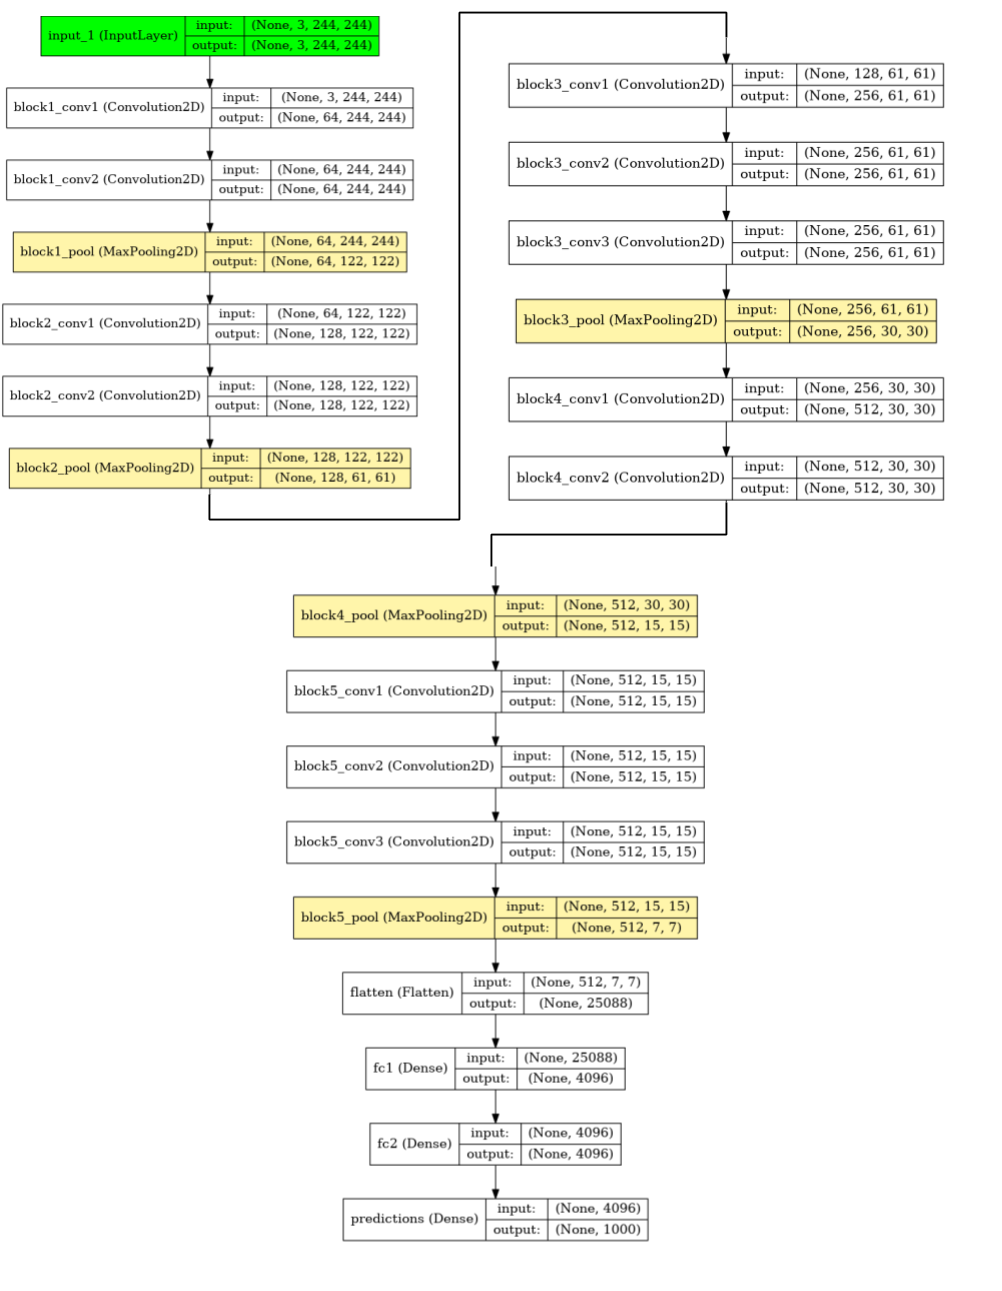
\includegraphics[width=0.9\textwidth]{./images/chapter5/vgg16.png}
  \caption[Πλήρες μορφή του δικτύου VGG16 της υλοποίησης]{Πλήρες μορφή του δικτύου VGG16 της υλοποίησης}
  \label{fig:vgg16}
\end{figure}

%% --------------------------------------------------------------------------
%\subsection{GoogleNet aka Inception-V1}

%\textbf{Να το προσθέσουμε και αυτό?}

%% --------------------------------------------------------------------------
\subsection{YOLO Net}

Το δίκτυο YOLO (You Only Look Once), είναι το πρώτο μοντέλο νευρωνικού δικτύου
συνέλιξης το οποίο προσπαθεί να επιλύσει το πρόβλημα της ταυτόχρονης αναγνώρισης
και εντοπισμού αντικειμένων σε εικόνες, με ένα προς-τα-εμπρός πέρασμα (forward pass).
Η ιδιαιτερότητά του είναι ότι αντιμετωπίζει το πρόβλημα σαν ένα πρόβλημα
regression και όχι classification.

Μία ακόμη ιδιαιτερότητα του συγκεκριμένου δικτύου είναι ότι θέτει σαν απαίτηση
την εφαρμογή του σε προβλήματα πραγματικού χρόνου και άρα στοχεύει κυρίως
στην ταχύτητα της αναγνώρισης. Φυσικά αυτό έχει σαν αποτέλεσμα την μείωση στην ακρίβεια
αναγνώρισης, η οποία είναι χαμηλότερη σε σχέση με άλλα μοντέλα, όπως για παράδειγμα τα δίκτυα
Fast-RCNN \cite{DBLP:journals/corr/Girshick15}, Overfeat και DetectorNet.

Η έξοδος του δικτύου αντιστοιχεί τόσο στις κλάσεις των αντικειμένων
που αναγνωρίστηκαν, καθώς και στις συντεταγμένες όπου και εντοπίστηκε.

\begin{figure}[!ht]
  \centering
  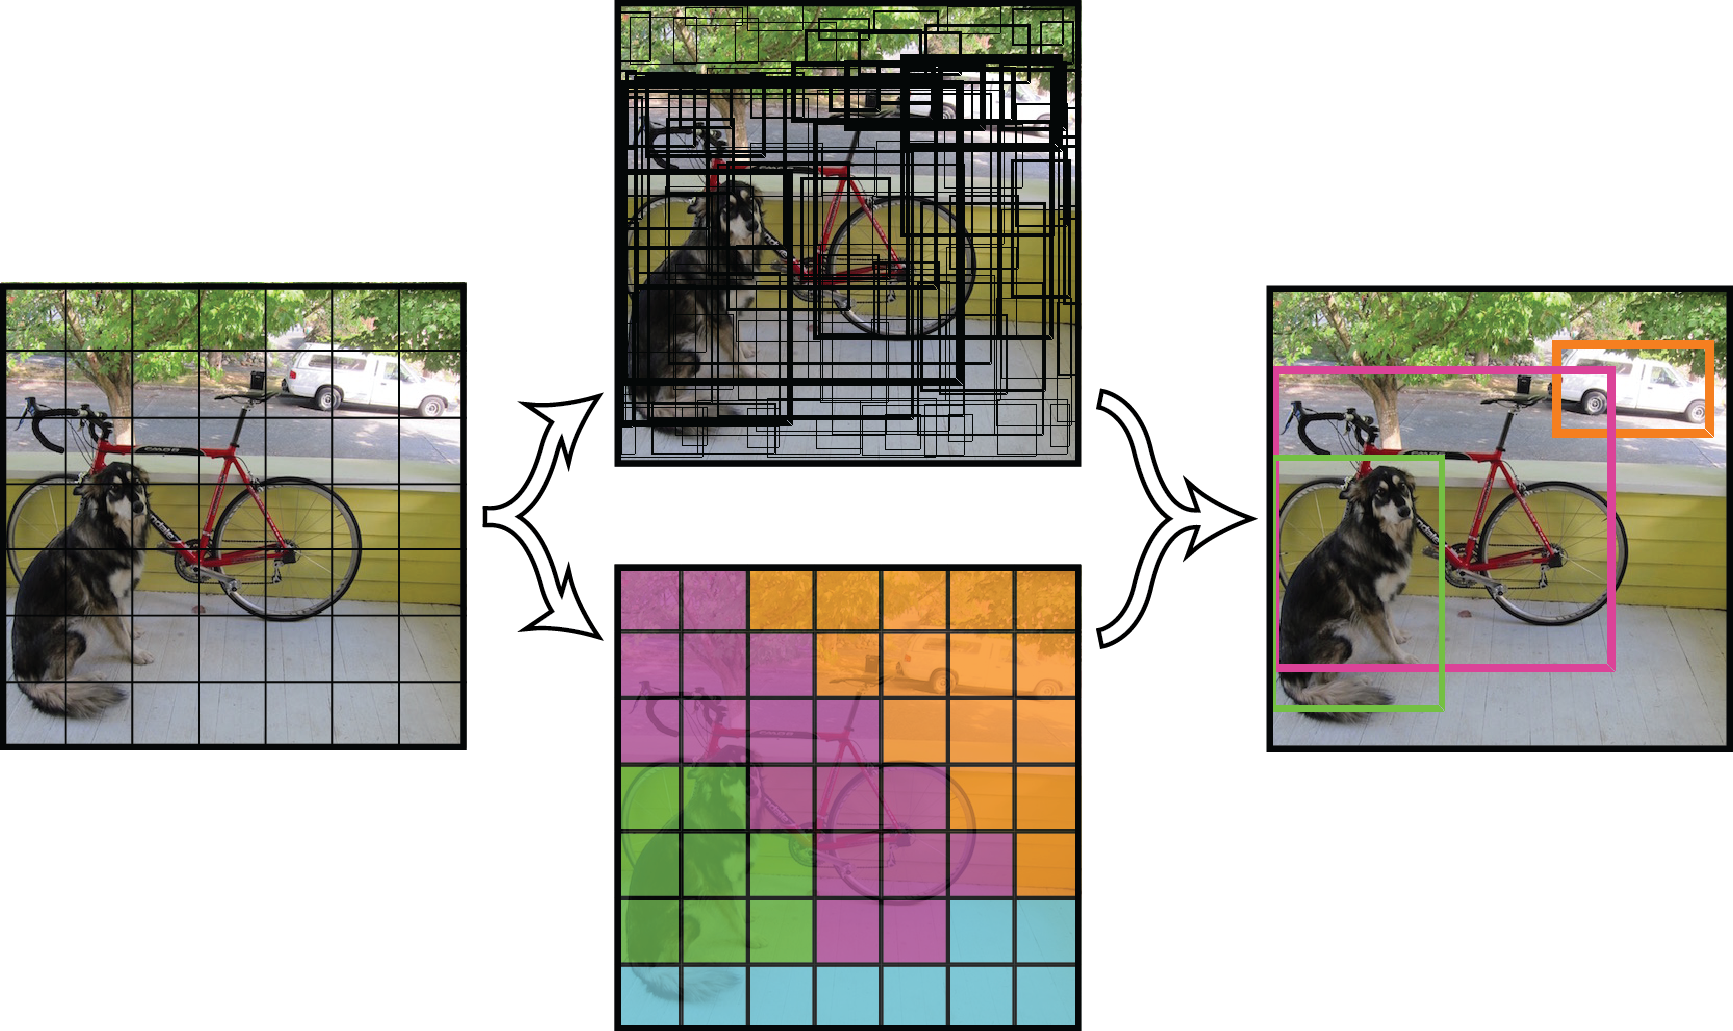
\includegraphics[width=0.8\textwidth]{./images/chapter5/yolonet_from_paper_1.png}
  \caption[Παράδειγμα τρόπου λειτουργίας του δικτύου YOLO]{Παράδειγμα τρόπου λειτουργίας του δικτύου YOLO}
  \label{fig:yolonet_from_paper}
\end{figure}

Το βασικό μοντέλο του δικτύου YOLO έχει την δυνατότητα να επεξεργάζεται εικόνες με ταχύτητα
\emph{45 fps} χρησιμοποιώντας μονάδα GPU (Nvidia Titan X).

Λόγω της ιδιαιτερότητας του συγκεκριμένου δικτύου, όσον αφορά τον τρόπο προσέγγισης του προβλήματος της ταυτόχρονης
αναγνώρισης και εντοπισμού των αντικειμένων, θεωρούμε σημαντικό να αναφέρουμε
και να εξηγήσουμε τον τρόπο λειτουργίας του.
Το πρώτο βήμα είναι να χωρίσει την εικόνα εισόδου σε ένα πλέγμα διαστάσεων $S \times S$
(αριστερή εικόνα στο \autoref{fig:yolonet_from_paper}).
Κάθε κελί του πλέγματος προβλέπει $B$ οριοθετημένα πλαίσια (bounding boxes) μαζί με ένα σκορ
"εμπιστοσύνης" για το κάθε πλαίσιο (πάνω μεσαία εικόνα στο \autoref{fig:yolonet_from_paper}).
Το σκορ εμπιστοσύνης ερμηνεύεται ως η βεβαιότητα
να ανήκει ένα αντικείμενο στο συγκεκριμένο πλαίσιο μαζί με την ακρίβεια ότι
το συγκεκριμένο αντικείμενο ανήκει σε αυτό το πλαίσιο. Η μαθηματική έκφραση
ορίζεται ως:
\begin{equation*}
  confidence = P(object | box = \imath) * IOU_{pred}^{truth}
\end{equation*}
Από την πιο πάνω μαθηματική έκφραση καταλαβαίνουμε ότι σε περίπτωση που
σε ένα κελί δεν υπάρχει αντικείμενο, το σκορ εμπιστοσύνης μηδενίζεται.
Επίσης, κάθε κελί του πλέγματος προβλέπει και τις πιθανότητες της κλάσης
του αντικειμένου, $P(class_{\imath} | object)$
(κάτω μεσαία εικόνα στο \autoref{fig:yolonet_from_paper}).

Χρησιμοποιώντας τις 2 αυτές μαθηματικές εκφράσεις των υπό-συνθήκη πιθανοτήτων,
καταλήγουμε στην σχέση
\begin{equation*}
  \begin{aligned}
    class-confidence = {} & P(class_{\imath} | object) * P(object | box = \imath) * IOU_{pred}^{truth} = \\
                          & P(class_{\imath}) * IOU_{pred}^{truth}
  \end{aligned}
\end{equation*}
η οποία μας δίνει το σκορ εμπιστοσύνης για μία συγκεκριμένη κλάση.

Κάθε οριοθετημένο πλαίσιο αποτελείται από πέντε προβλέψεις; $x, y, w, h$ και
το σκορ εμπιστοσύνης. Τα $x$ και $y$ αντιστοιχούν στις συντεταγμένες του
κέντρου του πλαισίου ενώ οι τιμές των $w$ και $h$ αναφέρονται στο
μήκος και το πλάτος του.

Τέλος, οι προβλέψεις στην έξοδο του δικτύου φαίνονται σαν ένας όγκος
διαστάσεων
\begin{equation*}
  S \times S \times (B * 5 + C)
\end{equation*}

Το πλήρες μοντέλο YOLO αποτελείτε από 24 επίπεδα συνέλιξης και 2 πλήρως
συνδεδεμένα.

Πέρα από το πλήρες μοντέλο, έχει σχεδιαστεί και εκπαιδευτεί, από την ίδια ομάδα ερευνητών, ένα μοντέλο
με παρόμοιο τρόπο λειτουργίας αλλά με πολύ λιγότερα επίπεδα συνέλιξης και άρα πιο
γρήγορο στην εκτέλεση (Tiny/Fast YOLO). Το TinyYOLO αποτελείτε από 9 επίπεδα
συνέλιξης και 2 πλήρες συνδεδεμένα. Σε όλα τα επίπεδα εκτός του τελευταίου
χρησιμοποιείται η συνάρτηση ενεργοποίησης LeakyReLU που παρουσιάστηκε στο \autoref{sec:theory_cnn}.

Η υλοποίηση μας στηρίχτηκε στην αντίστοιχη του μοντέλου Tiny-YOLO που έγινε από
την αντίστοιχη ερευνητική ομάδα \footnote{Βασική υλοποίηση του δικτύου YOLO: \url{http://pjreddie.com/darknet/}}
\cite{darknet13}.

Θεωρούμε σημαντικό να αναφέρουμε ότι αρχικά προσπαθήσαμε να τρέξουμε την βασική υλοποίηση,
η οποία είναι γραμμένη σε γλώσσα προγραμματισμού \emph{C}, ανεπιτυχώς.
Η εκτέλεση του προγράμματος υλοποίησης του μοντέλου Tiny-YOLO εμφανίζει σφάλματα
τύπου \emph{segmentation fault}.

\section{Βελτιστοποίηση των εργαλείων λογισμικού στο Jetson TK1}
\label{sec:implementations_jetson}

Στο \autoref{sec:jetson_tk1} είχαμε αναφέρει ότι η πλατφόρμα διαθέτει
λειτουργικό \emph{Linux4Tegra} το οποίο είναι ουσιαστικά διανομή Ubuntu 14.04
με εγκατεστημένους τους απαραίτητους drivers για το συγκεκριμένο σύστημα.

%προτού ξεκινήσουμε τις υλοποίησεις χρειάστηκε να εγκαταστήσουμε
%τα περισσότερα εργαλεία κατευθείαν πάνω στο μηχάνημα (build from source), για να αποφύγουμε
%την εγκατάστασή pre-compiled λογισμικού. Ο λόγος, όπως και θα φανεί στο \autoref{chapter:experiments},
%είναι ότι η απόδοση των συγκεκριμένων εργαλείων εξαρτάται τόσο από τις
%βιβλιοθήκες που θα χρησιμοποιηθούν για πράξεις γραμμικής άλγεβρας,
%όσο και από τις βελτιστοποιήσεις που γίνονται από τον μεταγλωττιστή κατά την
%διάρκεια της μεταγλώττισης του εκάστοτε πηγαίου κώδικά.

Ένα από τα πρώτα βήματα ήταν να απ-εγκαταστήσουμε από το λειτουργικό το
γραφικό περιβάλλον, για να περιορίσουμε την κατανάλωση μνήμης αφού η μνήμη
του ενσωματωμένου συστήματος Jetson TK1 είναι περιορισμένη στα 2 Gigabytes
και μάλιστα είναι κοινή μεταξύ των μονάδων GPU και CPU (shared memory).
Το γραφικό περιβάλλον Gnome
το οποίο είναι προεγκατεστημένο στην διανομή Linux4Tegra μετρήθηκε στα 114 Megabytes.
Το Jetson TK1 συνδέθηκε
μέσω θύρας ethernet στο δίκτυο ενός σταθερού υπολογιστή και έτσι ο χειρισμός
του έγινε μέσω καναλιού ssh\footnote{SSH: Secure Shell \href{https://tools.ietf.org/html/rfc4254}{{https://tools.ietf.org/html/rfc4254}}},
κερδίζοντας έτσι 114 Megabytes σε μνήμη. Αυτό το κέρδος, όπως θα φανεί
αργότερα, έπαιξε σημαντικό ρόλο, καθώς τα νευρωνικά δίκτυο που υλοποιήθηκαν
απαιτούν αρκετή μνήμη κατά την διάρκεια εκτέλεσής τους (της τάξης των Gigabytes).

Στην συνέχεια εγκαταστήσαμε τις βιβλιοθήκες CUDA και cuDNN για να εκμεταλλευτούμε
την υπολογιστική ισχύ της μονάδας GPU. Ο οδηγός για την εγκατάσταση βρίσκεται
στο %\href{http://elinux.org/Jetson_TK1}{http://elinux.org/Jetson_TK1}.
Επιπλέον έχουν γραφεί scripts σε \emph{Bash} για αυτόματη εγκατάσταση, τα
οποία είναι διαθέσιμα στο \emph{Github} στον σύνδεσμο %?????
%\href{https://github.com/klpanagi/Thesis/tree/master/jetson-tk1/}{https://github.com/klpanagi/Thesis/tree/master/jetson-tk1/}.

Ένα μεγάλο μέρος της συνεισφοράς της παρούσας διπλωματική εργασίας
ήταν να γίνουν βελτιστοποιήσεις σε επίπεδο λογισμικού των εργαλείων που χρησιμοποιήθηκαν
για το συγκεκριμένο μηχάνημα.

Αρχικά, ακολουθήσαμε τις οδηγίες για εγκατάσταση των εργαλείων \emph{numpy, scipy, Theano και Keras}
χρησιμοποιώντας τον επίσημο διαχειριστή πακέτων για Python, \emph{pip}.
Τα πρώτα αποτελέσματα σε χρόνους εκτέλεσης πράξεων γραμμικής άλγεβρας ήταν
απαγορευτικά (σχεδόν μία τάξη μεγέθους κάτω από το αναμενόμενο).
Τόσο η βιβλιοθήκη Theano, όσο και η numpy, χρησιμοποιούν εξωτερικές βιβλιοθήκες
για πράξεις γραμμικής άλγεβρας, οι οποίες ονομάζονται BLAS (Basic Linear Algebra Subprograms).

Καταλάβαμε ότι το πρόβλημα ήταν στους υπολογισμούς πράξεων γραμμικής άλγεβρας,
αφού σχεδόν όλες οι μαθηματικές εκφράσεις που εκτελούνται σε ένα
νευρωνικό δίκτυο είναι πράξεις πινάκων και εκτελέστηκε profiling των
ρουτινών BLAS χρησιμοποιώντας και τις τρεις βιβλιοθήκες που είναι διαθέσιμες για
επεξεργαστές ARM οι οποίες είναι οι εξής:
\begin{itemize}
  \item{libblas-dev + liblapack3 + libumfpack5.6.2: Προ-εγκατεστημένες στην διανομή Linux4Tegra}
  \item{ATLAS: Ανοικτού κώδικα}
  \item{OpenBLAS: Ανοικτού κώδικα}
\end{itemize}

Τόσο η βιβλιοθήκη ATLAS, όσο και η OpenBLAS, μεταγλωττίστηκαν από τον πηγαίο κώδικά τους,
λαμβάνοντας έτσι υπόψη τις απαραίτητες βελτιστοποιήσεις κατά την διαδικασία
της μεταγλώττισης. 
Συγκεκριμένα ορίσαμε στον μεταγλωττιστή να χρησιμοποιήσει την αρχιτεκτονική του
συγκεκριμένου επεξεργαστή (armv7) και τις μονάδες
NEON που διαθέτει, για τον υπολογισμό πράξεων με αριθμούς κινητής %?? what are NEON? ref or comment
υποδιαστολής \emph{ARM Cortex A15}. Επίσης ορίσαμε η εκτέλεση των ρουτινών
BLAS να γίνεται με πολυνηματικό τρόπο (4 threads).

Στην συνέχεια μετρήθηκε η απόδοση σε χρόνο εκτέλεσης των εξής ρουτινών BLAS:
\begin{itemize}
  \item{Εσωτερικό γινόμενο δύο διανυσμάτων με 1000 στοιχεία το καθένα}
  \item{Εσωτερικό γινόμενο δύο πινάκων διαστάσεων $1000 \times 1000$}
  \item{Αντιστροφή πίνακα διαστάσεων $1000 \times 1000$}
  \item{Υπολογισμός διακρίνουσας πίνακα διαστάσεων $1000 \times 1000$}
  \item{Υπολογισμός ιδιοτιμών πίνακα διαστάσεων $2000 \times 1000$}
  \item{Υπολογισμός ιδιοδιανυσμάτων πίνακα διαστάσεων $1500 \times 1500$}
\end{itemize}
Εκτελέστηκε κάθε μία από τις πιο πάνω ρουτίνες για 1000 επαναλήψεις και λήφθηκε
η μέση τιμή του χρόνου εκτέλεσης.
Οι καλύτεροι χρόνοι λήφθηκαν χρησιμοποιώντας την βιβλιοθήκη OpenBLAS.
Τα συγκριτικά αποτελέσματα μεταξύ της βιβλιοθήκης OpenBLAS και της προεγκατεστημένης
έχουν ως εξής: % add times instead of X times. Also put them in a table
\begin{itemize}
  \item{Εσωτερικό γινόμενο πινάκων: $\times 18$}
  \item{Εσωτερικό γινόμενο διανυσμάτων: καμία διαφορά}
  \item{Αντιστροφή πίνακα: $\times 11.5$}
  \item{Υπολογισμός διακρίνουσας πίνακα: $\times 9.6$}
  \item{Υπολογισμός ιδιοτιμών πίνακα: $\times 8.5$}
  \item{Υπολογισμός ιδιοδιανυσμάτων πίνακα: $\times 3.4$}
\end{itemize}
Αντίστοιχα, χρησιμοποιώντας την βιβλιοθήκη ATLAS πήραμε τα εξής αποτελέσματα:
\begin{itemize}
  \item{Εσωτερικό γινόμενο πινάκων: $\times 16$}
  \item{Εσωτερικό γινόμενο διανυσμάτων: $\times 1.5$}
  \item{Αντιστροφή πίνακα: $\times 10.2$}
  \item{Υπολογισμός διακρίνουσας πίνακα: $\times 7.4$}
  \item{Υπολογισμός ιδιοτιμών πίνακα: $\times 7.8$}
  \item{Υπολογισμός ιδιοδιανυσμάτων πίνακα: $\times 3.4$}
\end{itemize}

Αφού καταλήξαμε στην χρησιμοποίηση της βιβλιοθήκης OpenBLAS, συνεχίσαμε
με την μεταγλώττιση από πηγαίο κώδικα των βιβλιοθηκών numpy, scipy και Theano,
οι οποίες εκτελούν τις πράξεις BLAS, ορίζοντας αυτή την φορά στον μεταγλωττιστή
να χρησιμοποιήσει την συγκεκριμένη βιβλιοθήκη αντί της προ-εγκατεστημένης (link against shared library).

Τέλος, εγκαταστήσαμε στον Jetson TK1 την βιβλιοθήκη \emph{CNMeM}
\footnote{\href{https://github.com/NVIDIA/cnmem}{https://github.com/NVIDIA/cnmem}},
η οποία έχει αναπτυχθεί από την Nvidia και χρησιμοποιείται για την εκ των προτέρων
δέσμευση μνήμης σε μονάδες GPU που υποστηρίζουν CUDA.
Όπως θα φανεί στο επόμενο κεφάλαιο, η εκ των προτέρων δέσμευση μνήμης
επιταχύνει τον χρόνο εκτέλεσης. Ωστόσο απαιτεί σωστή ρύθμιση για να
αποφευχθούν περιπτώσεις δέσμευσης περισσότερης μνήμης από όση το
πρόγραμμα εκτέλεσης χρειάζεται.

Τέλος, είναι σημαντικό να αναφέρουμε ότι όλες οι προαναφερθέντες διαδικασίες εγκατάστασης των
εργαλείων λογισμικού καθώς και τα πειράματα που εκτελέσθηκαν περιγράφονται πλήρως στον
ιστοχώρο: %
\\

\href{https://github.com/klpanagi/Thesis/tree/master/jetson-tk1}{https://github.com/klpanagi/Thesis/tree/master/jetson-tk1}








\newevenside
\chapter{Πειράματα - Αποτελέσματα}
\label{chapter:experiments}

Τα πειράματα χωρίζονται σε δύο φάσεις. Στη πρώτη φάση τα CNN εκτελέστηκαν
σε έναν υπολογιστή με επεξεργαστή \emph{Intel i7 6700} και χωρητικότητα μνήμης
16GB. Στην συνέχεια, με βάση τα αποτελέσματα που λήφθηκαν στην πρώτη φάση των πειραμάτων, επιλέχθηκαν
τα αντίστοιχα μοντέλα CNN για να εκτελεστούν πάνω στην πλατφόρμα
Jetson TK1. Οι παράμετροι αξιολόγησης ήταν οι απαιτήσεις σε μνήμη και ο χρόνος εκτέλεσης
της διαδικασίας προς-τα-εμπρός περάσματος (forward propagation).

Για λόγους πληρότητας, πιο κάτω παρουσιάζονται τα βασικά χαρακτηριστικά
των δύο συστημάτων:
\\

\begin{table}
\small
\begin{tabular}{ | l | l | l | l | l | l | l | }
  \hline
  \rowcolor{Gray}
  Μηχάνημα & \# πυρήνων & \# νημάτων & clock & Κατ. Ισχύος & RAM & Cache \\
  \hline
  Host PC & 4 & 8 & 3.4 Ghz & ~65Watts & 16GB & 8MΒ L3 \\
  \hline
  TK1 & 4 & 4 & 2.32 & ~11Watts & 2GB (shared) & 2MB L2 \\
  \hline
\end{tabular}
\end{table}
Ο αριθμός νημάτων (8) που υποστηρίζει ο επεξεργαστής i7-6500 οφείλεται στην
υποστήριξη της τεχνολογίας \emph{Hyper-Threading}\footnote{\url{http://www.intel.com/content/www/us/en/architecture-and-technology/hyper-threading/hyper-threading-technology.html}}.
Σημαντικό επίσης να αναφέρουμε ότι η τιμή της κατανάλωσης ισχύος της
πλατφόρμας Jetson TK1, αντιστοιχεί στην κατάσταση μέγιστης λειτουργίας των μονάδων
CPU και GPU.

\section{Πρώτη Φάση Πειραμάτων}
\label{sec:experiments_phase1}

TODO!!

\section{Δεύτερη Φάση Πειραμάτων}
\label{sec:experiments_phase2}

TODO!!




\newevenside
\chapter{Συμπεράσματα}
\label{chapter:conclusions}

Στο κεφάλαιο αυτό παρουσιάζονται συνοπτικά οι υλοποιήσεις των μοντέλων CNN
και τα συμπεράσματα που προέκυψαν από την έκβαση των πειραμάτων.
Γίνεται σύγκριση της απόδοσης των μοντέλων αυτών στα δύο συστήματα
(PC με επεξεργαστή Intel i7-6700 και Jetson TK1), έχοντας ως
παραμέτρους αξιολόγησης τον χρόνο εκτέλεσης και την κατανάλωση ισχύος.
Στην συνέχεια αναφέρονται τα προβλήματα που παρουσιάστηκαν
κατά την διάρκεια των υλοποιήσεων και των πειραμάτων.

\section{Γενικά Συμπεράσματα}

Στα πλαίσια της παρούσας διπλωματικής εργασίας υλοποιήθηκε το δίκτυο
Tiny-YOLO χρησιμοποιώντας την βιβλιοθήκη Keras.
Τo δίκτυο AlexNet υλοποιήθηκε με βάση την αντίστοιχη υλοποίηση
στο Caffe \footnote{Υλοποίηση του δικτύου AlexNet στο Caffe: \url{https://github.com/BVLC/caffe/tree/master/models/bvlc_alexnet}},
και το μοντέλο του δικτύου VGG16 υπάρχει υλοποιημένο στα παραδείγματα του Keras.

Με βάση τα αποτελέσματα των πειραμάτων (βλ. \autoref{chapter:experiments})
που αφορούν στους χρόνους εκτέλεσης και κατανάλωσης ισχύος παρατηρήθηκαν τα
εξής:
\begin{itemize}
  \item{
      Οι καλύτεροι χρόνοι εκτέλεσης στον επεξεργαστή Intel-i7-6700 (και για τα 3 μοντέλα CNN)
      λήφθηκαν με χρήση τεσσάρων (4) νημάτων.
      Παρόλο που ο συγκεκριμένος επεξεργαστής υποστηρίζει (ψευδο)παράλληλη
      εκτέλεση 8 νημάτων (Hyper-Threading), παρατηρήθηκε στα πειράματα σημαντική
      καθυστέρηση. Το γεγονός αυτό οφείλεται στην εναλλαγή των νημάτων στους
      πυρήνες του επεξεργαστή
      (context switch\footnote{\url{http://wiki.osdev.org/Context_Switching}}).
    }
  \item{
      Ο χρόνος εκτέλεσης στην μονάδα CPU και των δύο συστημάτων παρουσιάζει αυξητικές διακυμάνσεις,
      ανάλογες προς τον αριθμό των νημάτων που εισέρχονται στον επεξεργαστή.
      Η αύξηση του αριθμού των νημάτων προσδίδει αβεβαιότητα στον χρόνο
      εκτέλεσης. Αντίθετα, ο χρόνος εκτέλεσης στην μονάδα GPU είναι γενικά σταθερός,
      χωρίς σημαντικές διακυμάνσεις και επομένως ενδείκνυται για εφαρμογές
      πραγματικού χρόνου.
      }
  \item{
      Με χρήση της βιβλιοθήκης CNMeM για εκ των προτέρων δέσμευση μνήμης
      ο χρόνος εκτέλεσης στην μονάδα GPU μειώνεται αισθητά (100-150ms).
    }
  \item{
      Η ισχύς που καταναλώνεται από την μονάδα GPU είναι σε κάθε περίπτωση χαμηλότερη σε σχέση
      με αυτή που καταναλώνει η μονάδα CPU σε κατάσταση μέγιστης
      λειτουργίας (χρήση τεσσάρων νημάτων).
    }
  \item{
      Με χρήση της μονάδας GPU ο χρόνος εκτέλεσης μειώνεται κατά
      2-5 φορές σε σχέση με την εκτέλεση στην μονάδα CPU του Tegra K1.
    }
  \item{
      Η εκτέλεση στην μονάδα GPU πέρα από το το γεγονός ότι είναι πιο γρήγορη,
      αφήνει 3.5 πυρήνες της μονάδας CPU ελεύθερες στο σύστημα.
      Αυτό είναι ιδιαίτερα σημαντικό αφού επιτρέπει την εκτέλεση άλλων
      διεργασιών (processes) στην μονάδα CPU.
    }
\end{itemize}

Επιπλέον, ο χρόνος εκτέλεσης της διαδικασίας forward propagation του
δικτύου Tiny-YOLO στο Jetson TK1 (0.3sec), είναι αποδεκτός
για χρήση του σε ρομποτικές εφαρμογές όπου δεν απαιτείται επεξεργασία
περισσότερων των τριών εικόνων το δευτερόλεπτο (3 frames per second). Αυτό
φυσικά εξαρτάται από τις απαιτήσεις της εκάστοτε εφαρμογής.


% ----------------------------------------------------------------------------

\section{Προβλήματα}

Ένα από τα αρχικά προβλήματα που παρουσιάστηκαν κατά την διάρκεια των υλοποιήσεων
ήταν η ασυμβατότητα μεταξύ των διαφόρων εργαλείων λογισμικού και του
ενσωματωμένου συστήματος. Συγκεκριμένα, τα εργαλεία για DL υποστηρίζουν σήμερα την 5η έκδοση της βιβλιοθήκης
\emph{cuDNN}, ενώ η τελευταία έκδοση που υποστηρίζεται για την μονάδα GPU που διαθέτει
το ενσωματωμένο σύστημα Jetson TK1 είναι η 2η. Αυτό έχει σαν αποτέλεσμα
τη μη ενσωμάτωση και χρήση της cuDNN από την βιβλιοθήκη Theano.

Ένα δεύτερο πρόβλημα ήταν η περιορισμένη μνήμη RAM που διαθέτει το
ενσωματωμένο σύστημα Jetson TK1. Παρόλο που το Tegra K1 SOC υποστηρίζει
μέχρι και 8GB μνήμη RAM η συγκεκριμένη πλακέτα διαθέτει μόνο 2GB.
Το γεγονός αυτό περιόρισε τον αριθμό των δικτύων που εκτελέστηκαν στο Jetson TK1
αφού δίκτυα με πολλά επίπεδα απαιτούν πολύ περισσότερη μνήμη. Συγκεκριμένα,
δοκιμάστηκε η εκτέλεση του δικτύου
ResNet σε PC και η μνήμη που απαιτούσε μετρήθηκε στα 3.7GB.
Η περιορισμένη μνήμη RAM έφερε προβλήματα και κατά την διαδικασία μεταγλώττισης
του δικτύου VGG16, τα οποία ωστόσο αντιμετωπίστηκαν προσθέτοντας μνήμη τύπου \emph{Swap}.



\newevenside
\chapter{Μελλοντικές επεκτάσεις}
\label{chapter:future_work}

Ένα από τα βασικά προβλήματα ήταν η περιορισμένη μνήμη που διαθέτει
το ενσωματωμένο σύστημα Jetson TK1 της Nvidia...


%\part{Πειράματα, Συμπεράσματα \& \\Μελλοντικές Επεκτάσεις}
%\part{Πειράματα, Συμπεράσματα \& Μελλοντικές Επεκτάσεις}
%\label{part:futurePart}
%\newevenside

  %\input{./chapters/chapter6_conclusions.tex}
  %\newevenside
  %\newevenside


%%%Bibliography

%\newevenside
%\newevenside
%\addcontentsline{toc}{chapter}{Βιβλιογραφία} %Added with tocbibind package
\renewcommand{\bibname}{Βιβλιογραφία}
\bibliography{./bibliography/general,./bibliography/deep_learning.bib,./bibliography/ai.bib,./bibliography/timings.bib,./bibliography/dnn.bib}

\end{document}

